\documentclass{article}
\usepackage{iclr2026_conference,times}
\input{math_commands.tex}

\usepackage{amsmath,amssymb}
\usepackage{booktabs}
\usepackage{array}
\usepackage{graphicx}
\usepackage{microtype}
\usepackage{xcolor}
\usepackage{placeins}
\usepackage{float}
\usepackage{longtable}
\usepackage{url}
\usepackage{hyperref}
\hypersetup{hidelinks}

\definecolor{shareblue}{RGB}{47,105,163}
\definecolor{copyorange}{RGB}{230,126,34}
\definecolor{mutegrey}{RGB}{90,90,90}
\newcommand{\qcomem}{\textsc{Q-CoMem}}
\newcommand{\method}{\textsc{ForkAudit}}
\newcommand{\materialize}{\textsc{Source+Materialize}}
\newcommand{\share}{\textsc{Shared-Document}}
\newcommand{\mib}{\,\mathrm{MiB}}
\newcommand{\gib}{\,\mathrm{GiB}}

\title{Q-CoMem: Quantized Split Replay for Memory-Constrained Hybrid LLMs}

\author{Anonymous authors}

% Anonymous ICLR submission: keep \iclrfinalcopy commented out.
% \iclrfinalcopy

\begin{document}
\raggedbottom
\maketitle

\begin{abstract}
Repeated queries over stable documents create a capacity problem: exact prefix
caching minimizes warm latency but retains state at every layer, whereas dense
recomputation retains nothing and reprocesses the document.  \qcomem{} is a capacity-first extension of CoMem split replay for hybrid LLMs:
an offline Write group-quantizes the depth-$j$ boundary residual with the
lower-layer KV, convolution and recurrent state later queries need, and online
Read dequantizes and forks it, keeps mutable request state private, and
replays the query before reconstructing the suffix.  A fail-closed \method{}
trace validates immutability, copy-on-write, recurrent rebinding, and call
provenance, because output equality alone can miss state aliasing; that
factorial runs full-prefix BF16 KV with no split depth and no quantization, so
it audits the ownership discipline and not the quantized Read path.

On an archival 60-item Qasper/2WikiMQA cohort with Qwen3.5-35B-A3B and H20-3e, a
frozen Q4/Q4/Q8 policy cuts mean retained tensor payload from $106.235$ to
$9.661$ MiB/document against a like-for-like all-BF16 reference ($10.9965\times$);
against the $136.235$ MiB the stack retains in native dtypes --- $30.000$ of it
FP32 GDN recurrent state in excess of BF16 --- the ratio is $14.10\times$, so
part is dtype narrowing, not packing.  Its mean F1 (0--100) against that same arm is
$54.24$ versus $54.68$, a paired difference of $-0.45$ $[-2.06,0.99]$ (10,000
paired item-level resamples, seed 20260902).  A separately executed run on the
same items adds a quantized exact cache: full-prefix Q8 retains $56.438$
MiB/document at $-3.78$ $[-9.12,0.32]$, so the frozen policy is $5.84\times$
smaller with a $3.41$-point higher mean F1, whose paired interval $-3.4122$
$[-8.4296,-0.0390]$ excludes zero by $0.0390$ points --- enough to support the
ordering, not to call the effect large or robust.  That arm stores every
attention layer at 8 bits against the frozen policy's 4, so the comparison is
not width-matched: the same component inventory rebuilds a width-matched exact
cache at $37.85$ MiB/document, and $5.84\times$ factors exactly into
$3.918\times$ from the split and $1.491\times$ from bit width.  No width-matched
exact cache was executed.  This is a selected
trade-off point among the evaluated policies, not selection-corrected, and not a
statistical-equivalence claim.  Timing is adverse.  On the 60-item
operating-point run full-prefix reaches the first token in $0.181$ s against
$0.656$ s for the frozen point and $0.636$ s for dense recomputation; on an
eight-item subset, median throughput falls from $13.38$ to $7.15$--$7.19$
tokens/s at TPOT within $2.5\%$ of $54.11$ ms --- point estimates over wide
per-repeat spread, since generation stops after a median of four to five tokens
rather than the 32-token cap, one per-repeat TPOT maximum reaches $404.01$ ms
against a $53.45$ ms median, and the throughput column reconciles with no
generated-token count, so we print minimum, median and maximum per timing cell
and read this evidence as weaker, not stronger.  On those same eight items,
SGLang~0.5.17 Radix reaches the first token in $0.146$ s and a published hybrid
prefix cache in $0.072$ s, both ahead of our $0.673$ s at the same $39.14$ mean
F1, while those arms retain $139.53$ and $324.09$ MiB/document against $15.89$.
The supported contribution is capacity reduction with an explicit online cost,
not TTFT acceleration.  Separately, at $N=32$ sharing one document's KV rather
than copying it per request lowers the
post-priming allocator delta from $4.901$ to $2.229\gib$ final ($54.5\%$) and
$4.920$ to $2.843\gib$ peak ($42.2\%$) --- but that full-copy arm is a
controlled ownership factor, not an optimized baseline, and against this paper's
own paged-prefix baseline the audited fork ties at $2.229/2.843\gib$ and is
worse on generation increment ($1.950$ versus $0.019\gib$), so it buys auditable
request-local state, not fewer allocator bytes.  The audit exposes a historical
alias that output and terminal-state equality miss but a persistent-base content
invariant also catches, so its increment is transition-time localization, not
exclusive detection.  We claim no lower total process memory, measured recall,
edge-device performance or broad quality preservation.
\end{abstract}

\section{Introduction}
\label{sec:intro}

Repeated queries over stable documents are common in document QA, agents, tree
search, and best-of-$N$ decoding.  Reusing a prefix avoids repeated prefill, but
exact caching retains per-document state at every layer, competing with weights,
request workspace, and other resident documents.  The question is
capacity-first: how much reusable state must stay resident, and what latency and
quality cost buys a smaller footprint?  Dense recomputation and exact caching are
the endpoints; CoMem instead writes a document to an intermediate depth and
reuses the per-token residual~\citep{liu2026comem,liu2026understanding}.  Hybrid
LLMs make this harder: lower full-attention layers also need KV, lower linear
layers need convolution and recurrent state, and those mutable states cannot be
shared blindly across requests~\citep{yang2025gateddeltanet,lieber2025jamba}.

\qcomem{} is a quantized hybrid split-replay design
(Figure~\ref{fig:qcomem-pipeline}) whose offline Write persists the split residual and all lower-layer state
a future query needs under state-type-aware low-bit packing, and whose online
Read dequantizes it, shares only immutable document tensors, creates
request-local mutable state, and reconstructs the suffix --- spending computation
to save retained bytes rather than trying to beat exact caching on TTFT.  Because
equal outputs can hide a mutable-state alias, we pair it with \method{}, a
phase-aware ownership trace over immutability, copy-on-write (COW), recurrent
rebinding, and call provenance, evaluated on a full-prefix BF16 configuration
rather than on the quantized Read path.  We contribute:
\begin{itemize}
  \setlength{\itemsep}{0pt}
  \setlength{\parskip}{0pt}
  \setlength{\topsep}{2pt}
  \setlength{\partopsep}{0pt}
  \item \textbf{Whole-entry accounting for a hybrid split-replay entry.}
Group-wise asymmetric quantization and per-layer, per-state-type width
assignment --- neither claimed as new (Section~\ref{sec:related}) --- applied to
an entry those methods do not address: the depth-$j$ residual \emph{together
with} the lower full-attention KV and convolution/recurrent state a hybrid
backbone needs.  CoMem retains only the residual, unquantized in BF16, so every
number here uses the whole-entry denominator
(Section~\ref{sec:decomposition}).
  \item \textbf{Memory, latency, and quality measured separately.} On 60
archived items the frozen Q4/Q4/Q8 point is $10.9965\times$ smaller than the
all-BF16 full-prefix reference ($14.10\times$ against the native-dtype entry the
stack retains) at $-0.45$ $[-2.06,0.99]$ mean F1; a separate run adds a
quantized exact cache, $5.84\times$ larger and $3.41$ points lower (paired
$-3.4122$ $[-8.4296,-0.0390]$, excluding zero at its edge) --- a ratio that is
not width-matched and factors into $3.918\times$ from the split and $1.491\times$
from bit width; and an eight-item execution reports TPOT and throughput with the
adverse TTFT trade-off visible against in-house and published same-stack systems
alike, under per-repeat dispersion we print rather than average away
(Sections~\ref{sec:memory}--\ref{sec:quality}).  Retained payload stays separate
from allocator and process memory, and Recall was measured in no cohort.
  \item \textbf{Ownership-safe reuse, audited off the quantized path.} The
seven-target \method{} contract couples semantic relations to phase-indexed
storage evidence across 96 ownership configurations, all full-prefix BF16 KV
with no split depth and no quantization; the quantized Read path is not audited.
A historical alias corrupts the persistent base while output and terminal
request state stay exact, but a persistent-base content invariant also catches
it, so the increment is transition-time localization, not exclusive detection.
Against our own paged-prefix baseline the audited fork ties at
$2.229/2.843\gib$ and is $1.950$ against $0.019\gib$ worse on generation
increment; the $54.5\%$/$42.2\%$ reduction at $N=32$ is against a full-copy
control, not that baseline (Section~\ref{sec:correctness}).
\end{itemize}

The timing execution uses an eight-item subset under its own generation
budget, the operating-point run a separate execution, and the ownership study
a third system entirely (Section~\ref{sec:setup}); ``Store'' is the
deduplicated sum of the tensor-storage bytes one entry owns, not total VRAM,
process memory, active workspace, or admitted capacity
(Sections~\ref{sec:denominators}, \ref{sec:limitations}).


\begin{figure}[t]
  \centering
  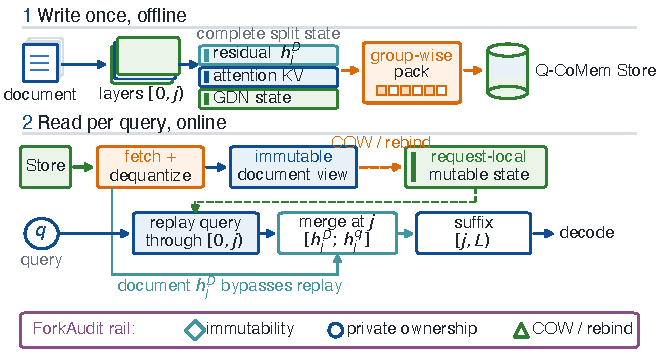
\includegraphics[width=0.81\textwidth]{figures/qcomem_pipeline_r47.pdf}
  \caption{\qcomem{} protocol geometry. Write packs the depth-$j$ residual with
the lower attention KV and GDN convolution/recurrent state; Read dequantizes
that entry, exposes immutable document tensors, creates request-local mutable
state through COW/rebinding, and replays the query through $[0,j)$ before the
suffix. The \method{} rail at the foot validates the ownership boundary and is
not an execution stage; it ran only on a full-prefix BF16 configuration with no
split depth and no quantization, so the packed Read path drawn here is
unaudited.}
  \label{fig:qcomem-pipeline}
\end{figure}

\section{Related Work}
\label{sec:related}

\paragraph{Split-depth reuse, paged and hybrid caching.}
CoMem persists one depth-$j$ residual per document token and replays the upper
suffix for later queries~\citep{liu2026comem,liu2026understanding}; we build on
that interface rather than claiming a new split-replay primitive, and add
quantizing the residual \emph{and} the lower KV/recurrent state a hybrid model
needs under an explicit storage denominator.  PagedAttention, Prompt Cache,
RadixAttention, ChunkAttention, Hydragen and Preble establish block sharing,
prefix reuse, shared-prefix computation and
scheduling~\citep{kwon2023pagedattention,gim2024promptcache,zheng2024sglang,
ye2024chunkattention,juravsky2024hydragen,srivatsa2025preble}: the low-TTFT
reference point, against which \qcomem{} trades suffix work for a smaller entry.
Gated Delta Networks maintain mutable compact
state~\citep{yang2025gateddeltanet}; Jamba, Marconi and HYPIC address hybrid
architectures or reusable hybrid
prefixes~\citep{lieber2025jamba,pan2025marconi,liu2026hypic} while storing that
state unquantized.  \method{} validates the immutable-document/mutable-request
boundary rather than replacing these policies, and
Table~\ref{tab:published-context} separates published numbers from our
controls.

\paragraph{KV and state quantization.}
Low-bit storage of reusable state is established prior art and \qcomem{} claims
none of its mechanisms.  The packer of Section~\ref{sec:write} is the standard
asymmetric affine quantizer~\citep{jacob2018quantization} applied group-wise, the
form FlexGen used for weights and the KV cache as 4-bit codes over 64-element
groups with per-group min/max metadata~\citep{sheng2023flexgen}; grouping-axis
choice, offline layer-wise mixed-precision assignment, rank or budget
allocation, and selective-SSM and recurrent-state quantization for hybrid
backbones are all established surfaces, attributed work by work in
Appendix~\ref{app:novelty-boundary}. Our bit vector $\mathbf b$ applies one of
them, not a new selection method.  What differs is the object: these methods pack one state family ---
attention keys and values --- produced on a single execution path, whereas a
hybrid split-replay entry mixes a boundary residual, lower-layer attention KV,
and mutable convolution and recurrent state, and we report Store for the whole
entry (Section~\ref{sec:decomposition}) rather than the residual alone, which
CoMem retains unquantized in BF16~\citep{liu2026comem}.

\paragraph{Quantized intermediates with recomputation.}
XQuant is the closest prior work to our core mechanism, and the distinction must
be stated in terms rather than by appeal to homogeneity: it caches quantized
layer-input activations and rematerializes keys and values during
decode~\citep{tomar2025xquant}, so persisting a quantized intermediate and paying
recomputation to avoid retaining downstream state is already its thesis.  Two things differ --- the cut point is a depth-$j$ boundary residual rather
than a layer input, and the retained object is a heterogeneous hybrid entry
rather than one state family, which is what raises the ownership question of
Section~\ref{sec:read} --- and Appendix~\ref{app:novelty-boundary} states both
in full. We claim the hybrid entry and its accounting, not
quantize-and-recompute.
Table~\ref{tab:closest} gives our boundary, and
Appendix~\ref{app:novelty-boundary} places the evaluation-methodology
precedents beside it.

\section{Motivation}
\label{sec:motivation}

A deployment must fit model weights, shared adapters, active workspace, retained
document entries, and runtime state at once:
\begin{equation}
 M_{\mathrm{device}} \geq M_{\mathrm{weights}}+M_{\mathrm{shared}}
 +M_{\mathrm{active}}+\sum_{D\in\mathcal{H}}S(D)+M_{\mathrm{runtime}},
 \label{eq:budget}
\end{equation}
where $\mathcal{H}$ is the hot document set. Weights and runtime are fixed once a model and stack are chosen, and
Eq.~\ref{eq:budget} multiplies the retained term by $|\mathcal{H}|$: the endpoints are dense recomputation, $S(D)=0$ at full prefill per query, and
exact caching, $136.235$ MiB/document here, with split replay at depth $j$
between them at the suffix-computation cost Section~\ref{sec:latency}
measures.  The workspace term is not
method-independent, and our own Read path is why: it materializes a private
dequantized copy of the entry per concurrent request (Section~\ref{sec:read}), so
$M_{\mathrm{active}}$ scales with the entry a method chose to retain, and we
print it for both arms instead of assuming it cancels.  \qcomem{} targets
$S(D)$: it does not compress weights or promise a smaller workspace, reports
allocator measurements under a separate denominator, and leaves process/NVML
memory unmeasured.

In a hybrid model that entry is not just larger but mutable: an honest
denominator counts the whole entry, and because those states are mutated in
place by the kernels that consume them, sharing one entry across concurrent
requests is an ownership question output comparison cannot answer. We observe
a historical configuration whose tokens and terminal request state stay exact
while a persistent base is corrupted, which a persistent-base content
invariant also catches, but only at final capture and without naming the
owner, layer, or family responsible (Section~\ref{sec:correctness}).

\section{Methodology}
\label{sec:method}

\subsection{Retained state decomposition}
\label{sec:decomposition}

For split depth $j$ the reusable hybrid state comprises the boundary residual
$h_j^D$, lower-layer full-attention KV, and lower-layer convolution/recurrent
state; with quantizer $Q_b$ the retained payload of Eq.~\ref{eq:budget} is
\begin{equation}
 S_{\mathrm{QCoMem}}(D;j,\mathbf b)=|Q_{b_h}(h_j^D)|+
 \sum_{\ell<j,\ell\in\mathcal A}|Q_{b_\ell}(K^D_\ell,V^D_\ell)|+
 \sum_{\ell<j,\ell\in\mathcal G}|Q_{b_\ell}(C^D_\ell,G^D_\ell)|,
\end{equation}
where $\mathcal A$ and $\mathcal G$ index full-attention and recurrent layers.
Counting only $h_j^D$ would understate the deployed state.  The bit vector $\mathbf b$ is assigned per state type and per layer.

\subsection{Offline Write: packing the complete entry}
\label{sec:write}

The document runs through layers $[0,j)$; we retain $h_j^D$ and the lower cache
leaves a later query needs, partitioning each floating tensor into 64-value
groups.  For a $b$-bit group with minimum $m$ and maximum $u$ we store
\begin{equation}
 s=(u-m)/(2^b-1),\qquad q=\operatorname{clip}
 \bigl(\operatorname{round}((x-m)/s),0,2^b-1\bigr),
 \label{eq:quant}
\end{equation}
with packed unsigned values and BF16 scale/bias metadata.  Three reimplementation details the equation omits --- the grouping axes and
their padding, the degenerate constant group, and the FP32 reconstruction path
--- are in Appendix~\ref{app:store-components}.

We write \emph{native dtype}, not ``Q16'', for the unpacked reference, because
that arm asserts no uniform width: BF16 residual and attention KV, the stack's
FP32 GDN recurrent state.  Every policy is one frozen bit vector with one name
here: \emph{frozen Q4/Q4/Q8} is a Q4 residual with cache widths $[8,8,8,4,8,8,8]$; \emph{calibrated per-layer} is a Q4 residual with
$[8,8,4,4,8,8,8]$, selected on a disjoint four-item calibration set under a byte
budget set by the frozen policy's predicted size; \emph{aggressive mixed} is a
Q4 residual with $[8,8,2,2,2,8,2]$, introducing the two-bit width, under a
budget $25\%$ below it.  Each is one frozen operating point, not a claim that
layer-wise selection is optimal.  Figure~\ref{fig:qcomem-quantization-map}
(Appendix~\ref{app:store-components}) separates these widths from the unchanged
BF16 model layers and forward computation.

\subsection{Online Read: ownership-safe fork and suffix replay}
\label{sec:read}

For each query the packed entry is dequantized into a logical document view.
For resident requests \(r\in\{1,\ldots,N\}\) the logical fork of that view is
\(\mathcal{F}_r(D)=\bigl(\{K^D_\ell,K^r_\ell\}_{\ell\in\mathcal A},
\{G^D_\ell,G^r_\ell\}_{\ell\in\mathcal G}\bigr)\), where document state
\(K^D_\ell,G^D_\ell\) is immutable and may be shared, whereas append
reservations \(K^r_\ell\) and mutable recurrent state \(G^r_\ell\) are
request-local. A borrowed recurrent base is read-only at setup and must rebind to private storage when
the registered transition first mutates it, and a partial KV tail is copied
before append. This discipline is what \method{} audits; the Transformers
implementation behind both deployment tables instead materializes a full
private copy of the dequantized entry per query, so it shares nothing and
exercises neither borrowing nor copy-on-write. Query tokens then traverse the
lower layers using request-local state; document and query residual chunks ---
distinct, as the Qwen3.5 recurrence requires --- seed the suffix through
$[j,L)$ before greedy decoding.

\subsection{Fail-closed validation of the ownership contract}
\label{sec:contract}

\method{} validates the ownership discipline of Section~\ref{sec:read} with
seven targets: frozen identity, prefix immutability, private ownership,
tail-safe COW, bounded host-side call provenance, cross-arm semantic
equivalence, and cross-\(N\) prefix consistency. It runs on a full-prefix BF16
configuration with no split depth and no quantization
(Section~\ref{sec:correctness}), so it validates that discipline and not the
dequantize-then-fork Read path; the packed-entry obligations ---
dequantized-view immutability, residual-chunk binding, packed-entry lifetime
--- are untested. A target passes only if its mandatory-slot coverage is
complete, every slot binds, and every replay predicate holds, so coverage is
separate from verdict; Appendix~\ref{app:storage-schema} gives that predicate
and the capture/replay workflow. Targets 2--5 are pre-output storage/call
obligations; 6--7 compare registered semantic observables and cannot
substitute for ownership evidence. It is an offline, non-adversarial
regression contract, not security attestation: capture/replay, the
mandatory-slot schema, slot-to-live-tensor binding and framework storage
semantics form the trusted computing base (TCB), and a pass establishes only
that the registered predicates held at captured points under it, covering
neither coherent omission/fabrication and transient writes between
observations nor compiled GDN, ATen/CUDA, or device/driver execution.

\section{Experiments}
\label{sec:experiments}
\label{sec:protocol}

\subsection{Setup and memory denominators}
\label{sec:setup}

\paragraph{Quality cohort and generation budgets.}
The broadest Store--F1 panel is an archival, raw-first validation run over 60
paired items --- Qasper and 2WikiMQA source indices 6--35, 30 per dataset ---
under official LongBench-v1 prompts and a 4,096-token input
cap~\citep{bai2024longbench,dasigi2021qasper,ho2020multihopqa}, comparing the
six policies of Table~\ref{tab:qcomem-validation60}.  Decoding is greedy with an EOS stop and a per-dataset budget of $128$
new tokens for Qasper and $32$ for 2WikiMQA; the operating-point run uses the
same budget and the eight-item panel $32$ for both, so the three panels' F1
levels are not interchangeable.  Four calibration prompts (indices 4--5) precede
and are disjoint from validation; the shards record no timing or Recall.  The stack is the one Table~\ref{tab:qcomem-tradeoff} names, on eight
H20-3e; the interpreter version was not recorded.  A separately executed
\emph{operating-point run} covers the same 60 items on it with one warm-up,
three repeats, and seed 20260903; it records TTFT and TPOT and adds a quantized
exact cache (full-prefix Q8: the same codec on the unsplit entry at a uniform
8-bit width, \emph{not} the frozen policy's bit vector) and a $j=13$ split
control.

F1 is our reimplementation of the LongBench-v1 \path{qa_f1_score} protocol, not
the upstream module, and two behaviours deviate --- an empty prediction or
reference scores $\mathrm{float}(\text{pred tokens}=\text{ref tokens})$, and
punctuation stripping is ASCII-only --- which we state because every F1 value,
delta and interval here depends on the scorer; citation~\citep{bai2024longbenchcode}
is the protocol source, not the code that produced these numbers.

\paragraph{Latency execution.}
A separate registered systems execution uses the same stack on eight items
(Qasper and 2WikiMQA source indices 6--9): a subset of the quality cohort's
\emph{items} but not of its measurement protocol, since it caps every arm at $32$
generated tokens.  That is why its full-prefix F1 reads $39.14$ against those
panels' $54.68$ and $54.67$ on a superset of the same items; the levels are not
comparable, and we do not decompose the gap into budget and item-difficulty
shares, because per-item F1 was not extracted under both protocols.

\paragraph{Memory denominators.}
\label{sec:denominators}
In both deployment tables ``Store'' is the deduplicated sum of the bytes of
the tensor storages one retained entry owns
(Appendix~\ref{app:store-components}), reported as a 60-item mean in
Table~\ref{tab:qcomem-validation60} and an eight-document median in
Table~\ref{tab:qcomem-tradeoff}.  It is \emph{not} the entry's physical byte-range union, which the same code
computes but does not print; that distinction was previously stated the other
way round, and Appendix~\ref{app:store-components} records that the correction
moves no number.
The whole $136.235$-versus-$140.34$ and $9.661$-versus-$10.01$ difference is
cohort and statistic, not length: document token counts are identical across the
operating-point run's arms and its own full-prefix mean Store matches the
archival cohort exactly, so we withdraw the earlier explanation of documents
$3.8\%$ longer: $69.3\%$ of the gap is which eight of the sixty documents the
timing panel draws and $30.7\%$ is a 60-item mean against an eight-item median,
with $0.0\%$ left to the estimand (Appendix~\ref{app:store-components}).  Neither denominator includes
non-tensor/Python metadata, allocator pools, process/NVML memory, active
workspace, or admission capacity; Section~\ref{sec:correctness} uses a third
denominator, and every quality difference uses the full-prefix arm of its own
execution.
Both deployment tables are Transformers-only executions of packed entries,
whereas Table~\ref{tab:rr2-memory} and every \method{} verdict come from a
different system --- vLLM~0.26 plus Transformers, full-prefix BF16 KV in
128-token pages, no split depth, no quantization, PG-19 --- so no \method{}
verdict here covers those packed entries.

\subsection{Memory: retained state per document}
\label{sec:memory}

Under the all-BF16 convention, which isolates packing from the stack's dtype
choices, splitting reduces mean Store from $106.235$ to $28.683$ MiB/document
($3.7038\times$) and the frozen Q4/Q4/Q8 policy to $9.661$, $10.9965\times$
below the reference.  The entry the
stack retains is larger, $136.235$ MiB/document, because it keeps GDN recurrent
state in FP32; $30.000$ of that is excess over a BF16 encoding, and against it
the same two steps read $3.93\times$ and $14.10\times$, so part of that physical
saving is dtype narrowing rather than the Eq.~\ref{eq:quant} packing step.  Both
columns are exact re-analyses of the same archived rows
(Appendix~\ref{app:store-components}).

The operating-point run supplies the arm the archival panel lacks: full-prefix
Q8, the unsplit entry at a uniform 8-bit width, retains $56.438$ MiB/document,
$2.41\times$ below the native-dtype reference but $5.84\times$ above the
frozen point. That ratio is not width-matched --- the frozen policy stores the
residual and the one lower attention layer at 4 bits, the exact-cache arm
every attention layer at 8 --- so we report its factors, not the product
alone: the component identity of Appendix~\ref{app:store-components} splits it
exactly into $37.846/9.661=3.9174$ from split depth and $56.436/37.846=1.4912$
from bit width, product $5.8416$, and only the $3.918\times$ is a split-replay
advantage, agreeing with the $3.93\times$ split step against the native-dtype
reference. \emph{No width-matched exact cache was executed}: the $37.85$ MiB
point is a byte count fixed by Eq.~\ref{eq:quant}'s format identity once the
bit vector is given, like the all-BF16 column, and we make no quality claim
for it. The method-dependent transient term of Eq.~\ref{eq:budget} is reported
for both arms in Appendix~\ref{app:store-components} rather than assumed to
cancel; it is arithmetic on Table~\ref{tab:store-components}, not an allocator
measurement, and fixes no concurrency limit.

\begin{table}[t]
\caption{Retained-state--quality trade-off on the 60-item validation cohort
(30 Qasper, 30 2WikiMQA) in two separate executions, blocked and never pooled,
each differenced against its own full-prefix row.  The all-BF16 columns come
first because they isolate packing from the stack's dtype choices.}
\label{tab:qcomem-validation60}
\centering\scriptsize
\setlength{\tabcolsep}{3.0pt}
\begin{tabular}{@{}lrrrrrrl@{}}
\toprule
\multicolumn{8}{@{}l}{\emph{Archival quality run (seed 20260902; no timing recorded)}}\\
Retained state & \multicolumn{2}{c}{Store, BF16 ref.} & \multicolumn{2}{c}{Store, native} & TTFT (s) & F1 (0--100) &
$\Delta$F1 vs. full-prefix [95\% CI] \\
 & MiB/doc & vs. & MiB/doc & vs. & & & \\
\midrule
No-cache dense recompute & -- & -- & -- & -- & & 54.29 & $-0.39$ [$-4.66$, $2.60$] \\
Full-prefix, native dtype & 106.235 & 1.00$\times$ & 136.235 & 1.00$\times$ & & 54.68 & $0.00$ [$0.00$, $0.00$] \\
\qcomem{} split, native dtype & 28.683 & 3.7038$\times$ & 34.683 & 3.93$\times$ & & 54.62 & $-0.06$ [$-0.18$, $0.00$] \\
\qcomem{} frozen Q4/Q4/Q8 & 9.661 & 10.9965$\times$ & 9.661 & 14.10$\times$ & & 54.24 & $-0.45$ [$-2.06$, $0.99$] \\
\qcomem{} calibrated per-layer & 9.395 & 11.3073$\times$ & 9.395 & 14.50$\times$ & & 53.36 & $-1.32$ [$-4.33$, $0.92$] \\
\qcomem{} aggressive mixed & 7.536 & 14.0969$\times$ & 7.536 & 18.08$\times$ & & 49.19 & $-5.50$ [$-11.58$, $-0.20$] \\
\midrule
\multicolumn{8}{@{}l}{\emph{Operating-point run (seed 20260903; separate execution on the same 60 items)}}\\
No-cache dense recompute & 0.000 & -- & 0.000 & -- & 0.636 & 54.18 & $-0.49$ [$-4.57$, $2.55$] \\
Full-prefix, native dtype & 106.235 & 1.00$\times$ & 136.235 & 1.00$\times$ & 0.181 & 54.67 & $0.00$ [$0.00$, $0.00$] \\
Full-prefix Q8 (uniform 8-bit) & 56.438 & 1.8823$\times$ & 56.438 & 2.41$\times$ & 0.182 & 50.89 & $-3.78$ [$-9.12$, $0.32$] \\
\qcomem{} frozen Q4/Q4/Q8, $j=13$ & 16.101 & 6.5980$\times$ & 16.101 & 8.46$\times$ & 0.582 & 51.27 & $-3.40$ [$-8.67$, $0.52$] \\
\qcomem{} frozen Q4/Q4/Q8, $j=7$ & 9.661 & 10.9965$\times$ & 9.661 & 14.10$\times$ & 0.656 & 54.30 & $-0.37$ [$-1.97$, $1.08$] \\
\bottomrule
\end{tabular}
\vspace{0.5mm}
\parbox{0.97\textwidth}{\scriptsize Store and F1 are 60-item means; each block uses its own full-prefix arm.
``Native'' keeps GDN recurrent state in FP32, ``BF16 ref.'' re-expresses it
(Appendix~\ref{app:store-components}).  Full-prefix Q8 packs the
unsplit entry at a uniform 8-bit width, \emph{not} the frozen policy's bit
vector, so the $5.84\times$ between it and the $j=7$ row is width-confounded
(Section~\ref{sec:memory}).  Decoding is
greedy at 128 new tokens for Qasper and 32 for 2WikiMQA; intervals are paired
10,000-resample item-level bootstrap percentile intervals against that block's
full-prefix arm (seeds 20260902/20260903) on unrounded means.  All ten pairwise
comparisons among the operating-point block's five arms, including the
frozen-versus-Q8 pair, are now computed and listed in
Appendix~\ref{app:all-intervals}; an interval crossing zero is not statistical
equivalence, the headline policy was selected without multiplicity adjustment,
and the ten pairs carry none either.  Recall was measured in no
cohort; blank TTFT cells mark a metric the archival run did not record.}
\end{table}


\subsection{Latency: TTFT, TPOT, and throughput}
\label{sec:latency}

\begin{table}[t]
\caption{The latency evidence, with the dispersion earlier versions of this panel
averaged away.  (a) The eight-item Qasper/2WikiMQA execution (source indices 6--9
of each dataset), every arm capped at 32 generated tokens, never pooled with the
60-item panels (Section~\ref{sec:setup}).  (b) The per-repeat spread of every
timing cell of the operating-point run.  Both use Qwen3.5-35B-A3B revision
\texttt{59d61f3}, PyTorch~2.11.0+cu129, Transformers~5.14.1, CUDA~12.9, one
H20-3e per item, a 4,096-token cap, greedy decoding and three timing repeats.}
\label{tab:qcomem-tradeoff}
\centering\scriptsize
\setlength{\tabcolsep}{3.0pt}
\begin{tabular}{@{}lrrrrrr@{}}
\toprule
\multicolumn{7}{@{}l}{\emph{(a) Eight-item execution; every cell a median over the eight documents, three repeats each}}\\
Retained state & Store (MiB/doc) & Reduction & TTFT (s) & TPOT (ms) & tok/s$^{\dagger}$ & F1 (0--100) \\
\midrule
No-cache dense recompute & 0.00 & -- & 0.649 & 648.75 & 1.36 & 39.42 \\
Full-prefix, native dtype & 140.34 & reference & 0.163 & 54.11 & 13.38 & 39.14 \\
\qcomem{} split Q8 & 15.89 & 88.68\% & 0.673 & 55.44 & 7.15 & 39.14 \\
\qcomem{} frozen Q4/Q4/Q8 & 10.01 & 92.87\% & 0.674 & 54.97 & 7.19 & 39.01 \\
\qcomem{} calibrated per-layer & 9.74 & 93.06\% & 0.673 & 55.07 & 7.19 & 39.11 \\
\qcomem{} split Q4 & 8.41 & 94.01\% & 0.674 & 55.02 & 7.19 & 36.09 \\
\bottomrule
\end{tabular}
\vspace{1.4mm}
\begin{tabular}{@{}lrrrrrrr@{}}
\toprule
\multicolumn{8}{@{}l}{\emph{(b) Operating-point run, 60 items $\times$ 3 repeats, seed 20260903; min / median / max over the three repeats}}\\
& \multicolumn{3}{c}{TTFT (s)} & \multicolumn{3}{c}{TPOT (ms)} & Median generated \\
Arm & min & med & max & min & med & max & tokens (cap 32) \\
\midrule
No-cache dense recompute & 0.2587 & 0.6482 & 1.4729 & 50.60 & 53.46 & 86.63 & 4 \\
Full-prefix, native dtype & 0.1500 & 0.1610 & 1.0891 & 50.53 & 53.45 & 404.01 & 4 \\
Full-prefix Q8 (uniform 8-bit) & 0.1545 & 0.1646 & 1.3874 & 50.73 & 53.46 & 89.93 & 5 \\
\qcomem{} frozen Q4/Q4/Q8, $j=13$ & 0.3192 & 0.5826 & 1.5740 & 51.51 & 54.18 & 89.34 & 4 \\
\qcomem{} frozen Q4/Q4/Q8, $j=7$ & 0.3527 & 0.6683 & 1.5296 & 51.56 & 54.19 & 86.84 & 4 \\
\bottomrule
\end{tabular}
\vspace{0.5mm}
\parbox{0.97\textwidth}{\scriptsize \emph{Aggregation.} Block (a) reports medians
over the eight documents and no dispersion, none having been recomputed for that
execution; block (b) the minimum, median and maximum of the three per-repeat
values.  Table~\ref{tab:qcomem-validation60}'s operating-point timing cells are
that run's recorded aggregates over the same 900 rows under a rule it did not
record, so they are not the block-(b) medians (full-prefix reads $0.181$ s there
against $0.161$ s here), though each falls inside the matching min--max range.
$^{\dagger}$Throughput is recorded, not derived: no single generated-token count
$n$ satisfies $n/(\mathrm{TTFT}+(n-1)\,\mathrm{TPOT})$ across block (a)
($n\approx5.3$ full-prefix, $7.3$--$7.4$ \qcomem{}, none at or above one token
for dense, whose own timings give $1.541$ tok/s at the cap against $1.36$
printed), and in the operating-point run the reconstruction from matched
per-repeat values still misses recorded throughput by a median $7.6$--$18.8\%$
per arm, so the column must not be inverted for a token count.  Store is the
deduplicated sum of the tensor-storage bytes one retained entry owns
(Section~\ref{sec:denominators}); block (a)'s reference is the entry in native
dtypes and every ``split'' arm retains a $j=7$ entry
(Appendix~\ref{app:store-components}); its calibrated per-layer row is smaller
and better than its frozen row, the opposite order to the 60-item panel
(Section~\ref{sec:quality}).  Recall was measured in no cohort.}
\end{table}


The eight-item timing characterization is not a speedup over exact caching
(Table~\ref{tab:qcomem-tradeoff}a): median TTFT rises from $0.163$ to
$0.673$--$0.674$ s on the \qcomem{} rows, which dequantize and rebuild the
suffix, and median throughput falls from $13.38$ to $7.15$--$7.19$ tokens/s at
TPOT within $2.5\%$ of $54.11$ ms.  The operating-point run sharpens the TTFT
comparison on all 60 items: full-prefix native dtype and Q8 reach the first
token in $0.181$ and $0.182$ s, dense recomputation in $0.636$ s, the frozen
$j=7$ point in $0.656$ s, so \qcomem{} is slower to the first token than honest
dense recomputation as well as than exact reuse, while TPOT stays between $54.4$
and $56.0$ ms at every arm.

\paragraph{What the dispersion does to all of that.}
As bare central values those cells concealed two facts, and readers were right
that no generated-token count reconciles the throughput column
(Table~\ref{tab:qcomem-tradeoff}, note~$\dagger$).  Panel~(b) prints the cause,
from the one execution whose per-repeat shards were retained: generation halts
after a median of four or five tokens under the protocol's EOS policy, so the
throughput denominator is four tokens and not the 32-token cap; and the
per-repeat spread is very large, TTFT maxima of $1.09$--$1.57$ s against medians
of $0.16$--$0.67$ s and a full-prefix TPOT maximum of $404.01$ ms against a
$53.45$ ms median.  Three consequences follow, each against us.  The $2.5\%$ TPOT
band compares point estimates whose repeat-level dispersion is unmeasured on that
panel and, where measured, far outside the band, so it is not a tolerance.  No
TTFT ordering is resolved by three repeats, every pair of min--max ranges in
panel~(b) overlapping.  And the ordering is unchanged at every aggregation we
computed and stays adverse: frozen $j=7$ is behind both exact caching and honest
dense recomputation.  We make no latency claim, and record that this dispersion
makes the timing evidence weaker, not stronger.

The comparison against deployed systems, not only our two in-house endpoints,
is harder.  On the identical eight items and
hardware, SGLang~0.5.17 Radix reaches the first token in $0.146$ s at $15.83$
tokens/s and the published HYPIC codebase's prefix cache in $0.072$ s at $19.07$
tokens/s, both at mean F1 $39.14$, against $0.673$--$0.674$ s and $7.15$--$7.19$
tokens/s at $39.01$--$39.14$ here (Tables~\ref{tab:h20-deployment},
\ref{tab:serving-controls}; within block).  Those arms retain a median $139.53$
and $324.09$ MiB/document against $15.89$ for \qcomem{} split Q8 --- three levels
we print rather than ratio, because the SGLang payload is quantized to 128-token
pages while ours is element-exact.  The supported result is a retained-capacity
trade-off with an explicit online cost and no latency advantage over any endpoint
we measured.


\subsection{Answer quality}
\label{sec:quality}

The frozen Q4/Q4/Q8 point has mean F1 $54.24$ versus $54.68$, a paired
difference of $-0.45$ $[-2.06,0.99]$ (10,000 paired item-level resamples, seed
20260902), negative on both datasets; the two steps compound rather than cancel,
splitting costing $-0.06$ and quantizing the split state a further $-0.39$, and
no item crosses the registered catastrophic threshold under either arm (0/60
against dense and against full-prefix).  The headline policy was selected among
six on this panel, so the interval is not selection-corrected and proves neither
equivalence nor noninferiority (Appendix~\ref{app:all-intervals}).

Against the operating-point run's full-prefix reference of $54.668$,
full-prefix Q8 scores $50.885$ ($-3.78$ $[-9.12,0.32]$) and the frozen $j=7$
point $54.297$ ($-0.37$ $[-1.97,1.08]$), so the frozen point is both
$5.84\times$ smaller than the only quantized exact cache we measured and
$3.41$ points higher in mean F1; that $5.84\times$ is the width-confounded
ratio Section~\ref{sec:memory} decomposes, and no width-matched arm exists to
say whether the F1 ordering survives at matched precision. The paired interval
between those two arms now exists: over the 60 common item keys, full-prefix
Q8 minus frozen $j=7$ is $-3.4122$ $[-8.4296,-0.0390]$ (10,000 paired
item-level resamples, seed 20260903), excluding zero, so the ordering is
supported on this cohort rather than merely observed. We claim that and no
more: the upper endpoint is $-0.0390$, near enough to zero that a different
resample sequence could carry it across, so the interval is evidence neither
that the effect is large nor that it is robust. Two neighbouring pairs from
the same pass fix the reading --- full-prefix at native dtype minus frozen
$j=7$ is $+0.3708$ $[-1.0533,+2.0345]$, the sign-reversed recomputation of the
$-0.37$ row above, and dense minus frozen $j=7$ is $-0.1173$
$[-4.4576,+3.1106]$, both crossing zero --- so the frozen point separates from
the quantized exact cache and from neither unquantized reference. All ten
pairs and their agreement with the printed rows are in
Appendix~\ref{app:all-intervals}. The $j=13$ control loses $3.40$
$[-8.67,0.52]$, nine times that loss, fixing the split depth at $j=7$ for this
policy --- one parameter, and we report nothing about depths this cohort did
not measure.

The two mixed policies are ablations, not improvements \emph{on the panel that
selects them}: the calibrated per-layer policy is named for its budget, not
measured parity, and the aggressive policy reaches $18.08\times$ with its
interval below zero and five threshold-crossing items
(Appendix~\ref{app:all-intervals}).  The eight-item panel orders the first pair
the other way, the calibrated policy being both smaller and better ($9.74$ MiB,
$39.11$, $\Delta=-0.022$) than the frozen point ($10.01$ MiB, $39.01$,
$\Delta\approx-0.13$ from the printed means), under a different budget and with no
interval; the 60-item cohort is the selector because it is larger, carries paired
intervals, and uses the full budget, and we report the inversion rather than the
favourable half of it.  Recall was recorded in no cohort and we make no recall
claim.

\subsection{Ownership and correctness validation}
\label{sec:correctness}
\label{sec:results}

\paragraph{Scope, cohort, and procedure.} \label{sec:target-status} The primary
factorial runs full-prefix BF16 KV on a vLLM-plus-Transformers stack with no
split depth and no dequantization step, and so audits the ownership discipline
of Section~\ref{sec:read}, not the quantized Read path of
Tables~\ref{tab:qcomem-validation60} and~\ref{tab:qcomem-tradeoff}.  Three executions produce the results below, each count naming its own
(Appendix~\ref{app:reproducibility};
Tables~\ref{tab:target-coverage}--\ref{tab:witness}).  All seven targets have
complete mandatory-trace coverage and pass at their declared fixed-stack scope,
with the live-binding rerun's stronger owner-row binding covering only one
selected cell (Section~\ref{sec:limitations}).  Every paired mutant is rejected
at its frozen gate while token equality and exact logits miss most of them, and
in a no-injection defect a persistent-base content invariant catches what output
and terminal state do not (Appendix~\ref{app:controls}), so the increment is
authenticated transition-time owner/layer/family localization, not exclusive
detection.  These and Appendix~\ref{app:controls}'s cohorts are fixed-case
comparisons against registered observables, not a detection study or an error
rate.

\paragraph{Allocator endpoints under a controlled ownership factor.}
Against the appropriate reference the ownership component saves nothing: at
$N=32$ the audited fork ties this paper's own paged-prefix baseline exactly
($2.229\gib$ final, $2.843\gib$ peak) and is $1.950$ against $0.019\gib$ worse
on generation increment, so it buys auditable request-local state, not fewer
allocator bytes.  The $54.5\%$/$42.2\%$ reduction is measured against a
different arm, a full-copy control that is a controlled ownership factor and not
an optimized baseline; Appendix~\ref{app:controls} prints both endpoints.

\subsection{Limitations and scope}
\label{sec:limitations}

The three panels sit on one Qwen3.5/H20 stack, none replicates another, none is
pooled, and they support bounded point estimates, not broad preservation.  The
archival run replays from raw outcomes but is not
source-frozen regeneration: its launcher used a mutable code directory, froze no
full-source or model-weight ledger, and left parts of its toolchain unarchived
(Appendix~\ref{app:reproducibility}); it has no timing, and no cohort measured
Recall.  H20 is not an edge device, so edge use is motivation, not an evaluated
claim; the calibrated per-layer row is one operating point from four disjoint
items; the split depth is validated against one alternative ($j=13$), not swept;
TTFT is higher than full-prefix reuse and, on the operating-point run, than
dense recomputation and the published prefix caches of
Section~\ref{sec:latency}; the timing panels are three repeats whose per-repeat
maxima reach $404.01$ ms TPOT against a $53.45$ ms median and whose generation
stops after a median of four to five tokens against a 32-token cap, so no timing
difference is resolved and the eight-item throughput column reconciles with no
generated-token count; that panel's dense TPOT of $648.75$ ms equals its own TTFT
to three digits, the re-prefill signature, against $53.46$ ms for the
operating-point run's prefill-once dense arm, a discrepancy we flag and do not
reconcile, its shards not being re-analysed; and we do not evaluate continuous
batching, QPS, admission, eviction, or scheduler effects.

Store, the deduplicated sum of the tensor-storage bytes one entry owns, excludes
non-tensor/Python metadata, allocator pools, active workspace, process/NVML
memory, and weights; reducing it does not by itself prove lower peak VRAM or
serving capacity, and the $54.5\%$/$42.2\%$ allocator result is a post-priming
delta against a full-copy control, neither additive with Store nor evidence of
higher admitted capacity.  The per-request transient of
Appendix~\ref{app:store-components} is likewise arithmetic, not an allocator or
NVML measurement, and fixes no concurrency limit for either arm.

\method{} has not been run on the quantized Read path: every ownership cell uses
full-prefix BF16 KV with no split depth or dequantization, whereas
Tables~\ref{tab:qcomem-validation60} and~\ref{tab:qcomem-tradeoff} measure a
$j=7$ packed Q4/Q4/Q8 path whose Read step materializes a full private copy
rather than borrowing it, so ownership there transfers by design argument only.
Within the TCB of Section~\ref{sec:contract} it upgrades semantic equality to
phase-indexed ownership evidence, but its selected-cell binding is a
same-process check: other cells and coordinates, framework/IPC semantics,
compiled GDN, ATen/CUDA, and device/driver execution stay unattested, and
constructed controls plus one historical mechanism show fixed-case sensitivity,
not population error rates (Appendix~\ref{app:expanded-limitations}).

\FloatBarrier

\section{Conclusion}

On 60 items the frozen Q4/Q4/Q8 point at $j=7$ is $10.9965\times$ smaller than
the all-BF16 full-prefix reference ($14.10\times$ native) at $-0.45$
$[-2.06,0.99]$, and $5.84\times$ smaller than a uniform-8-bit exact cache at
$3.41$ points better ($-3.4122$ $[-8.4296,-0.0390]$, excluding zero by $0.0390$
and no more) --- a width-confounded ratio factoring into $3.918\times$ from the
split and $1.491\times$ from bit width, no width-matched arm executed.  The cost
is explicit: exact reuse is faster in TTFT and higher in throughput, dense
recomputation and published prefix caches reach the first token sooner, and the
$2.5\%$ TPOT band is a point estimate whose per-repeat maximum reaches $404.01$
ms against a $53.45$ ms median, so no latency result is supported.  \method{}
localizes ownership violations on a full-prefix BF16 configuration, and the claim
is capacity-first: smaller retained state per document at bounded measured
quality, not Recall, total VRAM or faster inference.

\section*{Ethics Statement}
This work introduces no human-subject data collection. It uses public PG-19 text
for the trace-validation protocols and a fixed 60-item Qasper/2WikiMQA cohort,
whose eight-item subset carries the latency measurements. It does not assess
model safety, bias, privacy, or downstream deployment quality. Memory efficiency
can lower deployment cost but may also increase the scale of model use; those
broader effects are outside this controlled systems study.

\section*{Use of Large Language Models}
The authors used LLM-based assistance throughout: drafting and revising prose,
LaTeX, and tables; triaging related work; generating internal critiques and
revision plans that the authors adjudicated; and drafting experiment
specifications, including the registered response plan that selected which
additional runs this revision executed. Every experiment ran on
author-controlled infrastructure, and the authors verified each numerical claim
against the archived artifacts and take full responsibility for the content,
including any remaining errors.

\section*{Reproducibility Statement}
Claims map to registered evidence identifiers. The 60-item table maps to a
raw-first archival package that rechecks 66 mirrored files, 48 shards, 360
item-level F1 values, 24 paired-bootstrap intervals, and Store accounting; the
18 further intervals of Appendix~\ref{app:all-intervals} are recomputed from
those same archived per-item values, and the operating-point run's ten pairwise
intervals from its own archived rows at seed 20260903.
Table~\ref{tab:qcomem-validation60}'s operating-point block comes from a
separate registered execution (one warm-up, three repeats, seed 20260903) under
its own run identifier, not part of that package and never pooled with it. The
latency table is hash-bound to its eight workload shards and aggregate, and
manifest-first replay covers the primary ownership factorial and named
supporting cohorts. The research package accompanies this submission as
anonymous supplementary material, verified by content hash; it archives the
quantizer/split-replay module and the prompt-and-scoring driver
byte-identically, but not the panel runner, the launcher, the aggregation and
bootstrap scripts, the layer-policy search, or the deployment accountant, which
must be released before Table~\ref{tab:qcomem-validation60} is independently
re-executable. That table is therefore replayable from archived outcomes and not
re-executable today. Appendix~\ref{app:reproducibility} reports replay counts,
costs, non-reexecuted boundaries, and the unarchived parts of the 60-item
toolchain.

\bibliographystyle{iclr2026_conference}
\bibliography{references_r47}

\appendix

\section{Detailed Reproducibility and Artifact Scope}
\label{app:reproducibility}

The 60-item quality package (archive alias \textsc{qp-60}; manifest SHA-256
\path{24ac6952c6235bca6342171a9769f9da2d0e50d021e32c6ed453d931fd6c9952})
preserves 66 authoritative mirrored files from its recorded execution,
including 48 configuration-by-rank shards.  Its
raw-first verifier recomputes all 360 item-level F1 values, 24 paired-bootstrap
intervals, Store component accounting, and the archived aggregate.  The data
hash and policy receipt are bound and calibration precedes validation, but the
original execution did not freeze a complete source or model-weight ledger;
offline outcome replay therefore does not imply source-frozen GPU
regeneration.  The package archives the quantizer/split-replay module and the
prompt-and-scoring driver byte-identically at four paths, but not the run
driver, the aggregation and bootstrap scripts, the layer-policy search, the
deployment accountant, or the launch script; an artifact reviewer can therefore
read the code those files call but not the files that produced the table, and
they must be released before Table~\ref{tab:qcomem-validation60} is
independently re-executable.  The cohort is indexed against the LongBench-v1
release~\citep{bai2024longbenchrelease}, and F1 is our reimplementation of the
LongBench-v1 \path{qa_f1_score} protocol rather than the upstream module: the
citation~\citep{bai2024longbenchcode} is the protocol source, not the code that
produced any number in this paper, and the two behavioural deviations
(empty-prediction/empty-reference handling, ASCII-only punctuation stripping)
are stated in Section~\ref{sec:setup}.  Over-budget contexts keep their first
and last halves around the prompt's context marker, with a 256-token minimum.  The
archived receipt binds the prepared data file by content hash, but the upstream
dataset revision and evaluation-code commit were not recorded at execution time
and cannot be reconstructed after the fact; a re-executor must therefore match
the archived data hash rather than resolve an upstream revision.

\paragraph{What the seven targets establish.}
The primary rerun covers the $96$ frozen configurations of
Table~\ref{tab:protocol} on one
Qwen3.5-35B-A3B stack~\citep{qwen2026qwen35,qwen2026qwen35modelcard} and eight
PG-19 books~\citep{rae2020compressive}.
Every registered semantic observable matches exactly across the 96
configurations, and completed requests in both setup arms rebind at the
registered boundary to request-private tensors disjoint from the bases and from
completed peers.  The live-binding rerun's stronger owner-row binding covers only
the selected $N=8$ shared-document/materialized-GDN cell, leaving other cells and
the honest-process assumption outside it (Table~\ref{tab:v29-evidence-units}).

\paragraph{What a reader receives, and what is missing.}
The research package accompanies this submission as anonymous supplementary
material; every alias in Appendix~\ref{app:artifact} resolves inside it and is
verified by content hash.  Eleven components of the deployment stack are
recorded in the accompanying method-provenance table as \emph{not archived} in
any package: the split depth, all three bit policies and the layer-policy
search, the group-size verification, the 60-item panel runner and its launcher,
the Store accountant, the deployment accountant, the greedy/timing driver, and
the bootstrap and aggregation scripts.  Those are precisely the components that
select the reported operating point and produce the reported uncertainty, so
Tables~\ref{tab:qcomem-validation60} and~\ref{tab:qcomem-tradeoff} are
replayable from archived outcomes but not re-executable from the package, and we
state that here rather than only in a provenance file.

Manifest-first CPU replay covers the primary-factorial package and named
replayable supporting cohorts, not every contextual table.  The primary package
rechecks 536 artifacts, 96 cells, 288 cross-$N$ comparisons, eight attention
rows, and nine fault pairs.  The target-gate-suppression package rechecks 18
cases and 24 FP32 sidecars; its disclosed wrapper changes only an inherited
execution-identifier source and preserves every candidate byte.  The
independent-census package rechecks six IPC captures, 1,080 receiver rows,
96,660 relations, and omission/duplication/relabel controls against a
preproducer 180-slot expectation.  The dual-producer package binds two fresh
serial executions of the same frozen producer implementation and four distinct
observers, and rechecks exact zero-tolerance equality of the 1,080 observations
and 96,660 relation labels per execution.  The
bounded two-stream replay recomputes four full-logit comparisons and both
interval overlaps.

The fresh compiled-dispatch rerun binds a frozen source archive to a passing
eight-rank formal aggregate, eight rank receipts, 209,920 attention calls,
635,520 GDN calls, and 224 rejected post-run negative-control decisions.  The
local mirror preserves the primary and formal aggregates, runtime preflight,
raw/scientific ledgers, and both terminal ledgers; it does not duplicate the
model view or every raw shard.  The receipt closes target 5 only at the
declared honest-process fixed-stack boundary: normal launcher return is not a
device-side completion attestation, and compiled GDN, underlying ATen/CUDA
identity, and driver/device binaries remain outside scope.

The separate live-binding rerun binds a different frozen archive to eight
scientifically valid rank shards and a terminally complete formal tree.  Its
selected-cell hook validates 144 selected rows, 12,960 full live-storage rows,
3,840 direct clone edges, and 24 stable phase artifacts; a separately enumerated
schedule counter sees all 96 clean-memory calls with zero selected-context
overlaps.  The
post-run audit also rejects 184 formal controls and verifies 31 bytecode files,
13 descendant directories, and the 1,367-node final tree.  This supports only
the selected $N=8$ shared-document/materialized-GDN cell and six preregistered
owner-addressed rows per phase under an honest same-process runtime.

Within each selected witness call, the verifier (1) enumerates 60 persistent
sources before the builder, (2) records the actual builder's persistent-rooted
Torch-dispatch clone edges, (3) exhaustively matches 480 destinations and passes
a one-use capability bound to the exact group and verifier, (4) rereads all 540
live tensors against the production serializer at three phases, and (5)
publishes hash-bound phase paths for terminal reread.  Any count, object,
descriptor, lineage, phase-order, or path mismatch aborts before acceptance.
Trusted components are hook placement, Python/Torch-dispatch and tensor/storage
semantics, and honest process scheduling; group identity, object continuity,
lineage cardinality, serializer fields, and publication paths are checked.

The designer--executor-separated package binds the PDF-only author freeze, a
lifecycle-amended executor, five clean/mutant pairs, detached clean and pair
replays, and 208 terminal files.  All five clean gates and expected-first
classifications pass; the pre-injection amendment was frozen before all five
ranks were rerun in a new output root.

The historical-regression package binds the pre-discovery chronology, frozen
pre-fix/repair sources, outcome-blind protocol and resource amendment, eight
three-lane rank artifacts, 24 FP32-logit sidecars, and 24 fresh nonces.  A fresh
candidate-import-free replay of every rank and the aggregate is byte-identical
to the archived output.

The expanded numerical-sweep package binds 272 sidecars totaling 140,199,936
bytes and rechecks 20 attention and 24 GDN clean rows plus 44 controls.  The
Falcon package compares candidate arms against a separately executed official
Transformers reference on 8 ranks and detached-replays the aggregate.  HYPIC
binds 4,404 timing artifacts and hash-replays all 16 Store cells.  No package
enumerates OS/driver allocations; every conclusion remains bounded to its
declared configuration.  Appendix~\ref{app:artifact} maps exact artifacts and
boundaries.

On one Apple-silicon (M4-class) laptop CPU host, three consecutive fixed-order
replays without a
cache flush took a median 100.146\,s (99.248--110.526\,s) for the core package
and 105.717\,s (104.846--119.566\,s) for the serial profile that additionally
ran five locally complete supporting verifiers; the paired within-profile
increment was 5.598\,s (5.571--9.039\,s).  The canonical core distribution has
630 files and 892,284,156 logical bytes (850.95\,MiB); 536 raw traces occupy
888,785,811 bytes, or 99.62\% of manifest-payload bytes.  These are local CPU
replay and logical-storage measurements, not H20 capture cost, GPU perturbation,
cold-start latency, online inference cost, or a matched uninstrumented delta.

\section{Complete Interval Inventory and the Reference-Arm Change}
\label{app:all-intervals}

Every paired-bootstrap interval that exists for the 60-item panel is listed
here, so that none is computed but unreported. The archival analysis computed
24 intervals: six configurations against dense and against split, native dtype
pooled (12), and six configurations against dense on each dataset (12).
\emph{None used the native-dtype full prefix as its reference arm}, although
the Store column and every compression ratio in
Table~\ref{tab:qcomem-validation60} do. This revision therefore recomputes 18
further intervals against the native-dtype full prefix --- six configurations
$\times$ pooled/Qasper/2WikiMQA --- from the same 360 archived item-level F1
values, and Table~\ref{tab:qcomem-validation60} now displays the six pooled
ones. It also adds all ten pairwise comparisons among the operating-point
run's five arms, the block that previously reported only differences against
its own full-prefix reference. No measurement was repeated: the recomputation
reproduces all six published mean-F1 values and all five published Store
values exactly (the largest deviation of any recomputed point estimate from
the archived one is $6.11\times10^{-16}$ F1 points), and reproduces the
archived intervals to within Monte-Carlo noise. The archived analysis records
no bootstrap seed, so its endpoints are reproducible only up to that noise;
the new intervals use seed 20260902, 10,000 paired item-level resamples of the
60 common $(\mathrm{dataset},\ \mathrm{source\ index})$ keys, and a percentile
interval. Because seed plus resample count does not fix percentile endpoints
across RNG libraries, we state the generator: a Python \path{random.Random}
seeded once per comparison, drawing resample indices one at a time in
$\mathrm{randrange}(n)$ order, with the reported endpoints taken as the order
statistics at indices $\lfloor 0.025(n-1)\rfloor$ and $\lfloor
0.975(n-1)\rfloor$ of the sorted resampled means. Endpoints reproduce exactly
only for this generator, seed sequence, and repetition count. Across five
seeds the frozen row's endpoints move by at most $0.075$ points, so the
intervals are quoted to two decimals.

Two consequences of the change of arm are worth stating.  First, the two steps
compound rather than cancel: $-0.0585$ for splitting plus $-0.3870$ for
quantizing the split state equals the $-0.4455$ reported against full-prefix,
so the previously published $-0.39$ understated the deployment-relevant loss by
about $13\%$ of its value.  Second, the frozen policy's registered safety count
is unchanged by the change of arm: $0/60$ items below the $-50$-point
catastrophic threshold against dense and $0/60$ against full-prefix.

The ten operating-point pairs come from a separate pass over that run's 60
common item keys, 10,000 paired item-level resamples at seed 20260903, and the
same generator and percentile convention.  Their point estimates reproduce the
four differences Table~\ref{tab:qcomem-validation60} prints against the
full-prefix arm exactly, and their endpoints agree with the printed ones to
within $0.20$ F1 points --- the resampling noise of an independently drawn
resample sequence, of the same order as the $0.075$-point five-seed movement
recorded above.  One pair, full-prefix Q8 minus frozen $j=7$ at $-3.4122$
$[-8.4296,-0.0390]$, excludes zero; the other nine do not.  That one is the
comparison earlier revisions declined to compute, and its upper endpoint lies
$0.0390$ points from zero, so it supports the ordering and nothing about the
size or the robustness of the effect.  None of the ten carries a multiplicity
adjustment, and none is an equivalence or noninferiority test.
Two ablation details from Section~\ref{sec:quality} belong with this inventory:
on the 60-item panel the calibrated per-layer policy saves $2.75\%$ Store while
its mean-F1 difference is more negative than the frozen point's and one of 60
items crosses the catastrophic threshold, and uniform Q4 loses $3.047$ points on
the eight-item execution.

\paragraph{Why dense is not the per-item reference.}
The archived rows show identical prefix, document, query and input token
counts, identical truncation flags, and identical items, questions and
references across all six arms, so the wide dense interval is not an
execution-boundary artifact.  What the rows do show is that dense
recomputation and cached-prefix continuation emit different greedy token
sequences on 6 of 60 items, two of them short-answer 2WikiMQA questions whose
per-item F1 is nearly binary; the per-item difference standard deviation is
$14.51$ against $0.45$ for full-prefix versus split at native dtype, which is why the
interval is $41\times$ wider.  Logits are not archived, so we report the
divergence rather than asserting its mechanism.  By the same measure
\qcomem{} split replay at native dtype tracks the full-prefix reference more closely ($58/60$ identical
token sequences) than dense recomputation does ($54/60$), and on both items
where it differs its output is the one that matches dense.  The dense row is
therefore retained as a no-retention reference, not as a per-item baseline.

\begingroup
\footnotesize
\setlength{\LTpre}{4pt}
\setlength{\LTpost}{4pt}
\begin{longtable}{@{}>{\raggedright\arraybackslash}p{0.30\linewidth}llr@{}}
  \caption{All 52 paired-bootstrap intervals for the 60-item panels, on the
  $0$--$100$ F1 scale.  The first block is the 18 intervals computed against the
  native-dtype full prefix on the archival run (seed 20260902); the second is
  the operating-point run's ten pairwise comparisons (seed 20260903), which
  complete that block's inventory; the third is the 24 intervals in the archival
  analysis, with the reference arm each one actually used.  Rows in the first
  block with a pooled subset are the ones displayed in
  Table~\ref{tab:qcomem-validation60}.}
  \label{tab:all-intervals}\\
  \toprule
  Configuration & Subset & $\Delta$F1 & 95\% CI \\
  \midrule
  \endfirsthead
  \multicolumn{4}{c}{\textit{Table~\ref{tab:all-intervals} continued.}}\\
  \toprule
  Configuration & Subset & $\Delta$F1 & 95\% CI \\
  \midrule
  \endhead
  \midrule
  \multicolumn{4}{r}{\textit{Continued on next page}}\\
  \endfoot
  \bottomrule
  \endlastfoot
  \multicolumn{4}{@{}l}{\emph{This revision; reference arm: full-prefix, native dtype (18 intervals)}}\\
  No-cache dense recompute & pooled & $-0.3934$ & [$-4.6648$, $+2.6049$] \\
  No-cache dense recompute & Qasper & $+1.2131$ & [$-0.2339$, $+3.3305$] \\
  No-cache dense recompute & 2WikiMQA & $-2.0000$ & [$-10.0000$, $+4.0000$] \\
  Full-prefix, native dtype & pooled & $+0.0000$ & [$+0.0000$, $+0.0000$] \\
  Full-prefix, native dtype & Qasper & $+0.0000$ & [$+0.0000$, $+0.0000$] \\
  Full-prefix, native dtype & 2WikiMQA & $+0.0000$ & [$+0.0000$, $+0.0000$] \\
  \qcomem{} split, native dtype & pooled & $-0.0585$ & [$-0.1754$, $+0.0000$] \\
  \qcomem{} split, native dtype & Qasper & $-0.1170$ & [$-0.3509$, $+0.0000$] \\
  \qcomem{} split, native dtype & 2WikiMQA & $+0.0000$ & [$+0.0000$, $+0.0000$] \\
  \qcomem{} frozen Q4/Q4/Q8 & pooled & $-0.4455$ & [$-2.0586$, $+0.9907$] \\
  \qcomem{} frozen Q4/Q4/Q8 & Qasper & $-0.3354$ & [$-3.3818$, $+2.3932$] \\
  \qcomem{} frozen Q4/Q4/Q8 & 2WikiMQA & $-0.5556$ & [$-1.6667$, $+0.0000$] \\
  \qcomem{} calibrated per-layer & pooled & $-1.3174$ & [$-4.3322$, $+0.9193$] \\
  \qcomem{} calibrated per-layer & Qasper & $-0.2539$ & [$-3.3148$, $+2.3720$] \\
  \qcomem{} calibrated per-layer & 2WikiMQA & $-2.3810$ & [$-7.1429$, $+0.0000$] \\
  \qcomem{} aggressive mixed & pooled & $-5.4961$ & [$-11.5805$, $-0.1984$] \\
  \qcomem{} aggressive mixed & Qasper & $-3.9445$ & [$-11.4709$, $+1.5691$] \\
  \qcomem{} aggressive mixed & 2WikiMQA & $-7.0476$ & [$-17.7143$, $+1.3333$] \\
  \midrule
  \multicolumn{4}{@{}l}{\emph{Operating-point run; all ten pairwise comparisons, pooled (seed 20260903)}}\\
  Dense $-$ full-prefix, native dtype & pooled & $-0.4881$ & [$-4.5660$, $+2.5509$] \\
  Dense $-$ full-prefix Q8 & pooled & $+3.2949$ & [$-2.4786$, $+9.4520$] \\
  Dense $-$ frozen Q4/Q4/Q8, $j=13$ & pooled & $+2.9071$ & [$-2.8268$, $+8.9943$] \\
  Dense $-$ frozen Q4/Q4/Q8, $j=7$ & pooled & $-0.1173$ & [$-4.4576$, $+3.1106$] \\
  Full-prefix, native dtype $-$ full-prefix Q8 & pooled & $+3.7831$ & [$-0.1914$, $+9.3195$] \\
  Full-prefix, native dtype $-$ frozen, $j=13$ & pooled & $+3.3952$ & [$-0.5737$, $+8.7639$] \\
  Full-prefix, native dtype $-$ frozen, $j=7$ & pooled & $+0.3708$ & [$-1.0533$, $+2.0345$] \\
  Full-prefix Q8 $-$ frozen Q4/Q4/Q8, $j=13$ & pooled & $-0.3878$ & [$-5.3363$, $+4.6122$] \\
  \textbf{Full-prefix Q8 $-$ frozen Q4/Q4/Q8, $j=7$} & pooled & $\mathbf{-3.4122}$ & [$\mathbf{-8.4296}$, $\mathbf{-0.0390}$] \\
  Frozen $j=13$ $-$ frozen $j=7$ & pooled & $-3.0244$ & [$-8.2344$, $+0.5789$] \\
  \midrule
  \multicolumn{4}{@{}l}{\emph{Archival analysis; reference arm as listed (24 intervals)}}\\
  \midrule
  Configuration & Reference arm & Subset & 95\% CI \\
  \midrule
  No-cache dense recompute & dense & pooled & [$+0.0000$, $+0.0000$] \\
  No-cache dense recompute & split, native dtype & pooled & [$-4.6063$, $+2.6650$] \\
  No-cache dense recompute & dense & 2WikiMQA & [$+0.0000$, $+0.0000$] \\
  No-cache dense recompute & dense & Qasper & [$+0.0000$, $+0.0000$] \\
  Full-prefix, native dtype & dense & pooled & [$-2.6066$, $+4.5088$] \\
  Full-prefix, native dtype & split, native dtype & pooled & [$+0.0000$, $+0.1754$] \\
  Full-prefix, native dtype & dense & 2WikiMQA & [$-4.0000$, $+10.0000$] \\
  Full-prefix, native dtype & dense & Qasper & [$-3.3305$, $+0.2339$] \\
  \qcomem{} split, native dtype & dense & pooled & [$-2.6650$, $+4.4572$] \\
  \qcomem{} split, native dtype & split, native dtype & pooled & [$+0.0000$, $+0.0000$] \\
  \qcomem{} split, native dtype & dense & 2WikiMQA & [$-4.0000$, $+10.0000$] \\
  \qcomem{} split, native dtype & dense & Qasper & [$-3.4475$, $+0.0000$] \\
  \qcomem{} frozen Q4/Q4/Q8 & dense & pooled & [$-3.3045$, $+4.2800$] \\
  \qcomem{} frozen Q4/Q4/Q8 & split, native dtype & pooled & [$-2.0365$, $+1.0756$] \\
  \qcomem{} frozen Q4/Q4/Q8 & dense & 2WikiMQA & [$-4.3333$, $+9.4444$] \\
  \qcomem{} frozen Q4/Q4/Q8 & dense & Qasper & [$-4.6073$, $+0.7317$] \\
  \qcomem{} calibrated per-layer & dense & pooled & [$-5.2845$, $+3.7838$] \\
  \qcomem{} calibrated per-layer & split, native dtype & pooled & [$-4.2793$, $+0.9775$] \\
  \qcomem{} calibrated per-layer & dense & 2WikiMQA & [$-8.4762$, $+8.6667$] \\
  \qcomem{} calibrated per-layer & dense & Qasper & [$-4.9649$, $+1.6662$] \\
  \qcomem{} aggressive mixed & dense & pooled & [$-11.9941$, $+1.5786$] \\
  \qcomem{} aggressive mixed & split, native dtype & pooled & [$-11.5615$, $-0.1713$] \\
  \qcomem{} aggressive mixed & dense & 2WikiMQA & [$-16.7619$, $+6.6667$] \\
  \qcomem{} aggressive mixed & dense & Qasper & [$-12.9395$, $+1.0689$] \\
\end{longtable}
\endgroup

\section{Per-Component Store Accounting and the Format Ceiling}
\label{app:store-components}

\begin{figure}[H]
  \centering
  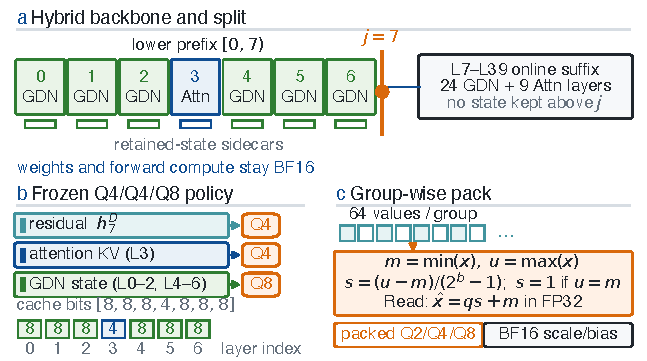
\includegraphics[width=0.85\textwidth]{figures/qcomem_quantization_map_r47.pdf}
  \caption{Quantization scope and the frozen Q4/Q4/Q8 policy. (a) At split
$j=7$ the retained entry holds the boundary residual and the lower-layer
(L0--L6) state sidecars; weights and forward computation stay BF16, and
L7--L39 state is reconstructed on Read. (b) The frozen policy's cache bit
vector is $[8,8,8,4,8,8,8]$ with a Q4 residual: $h_7^D$ and the L3 attention KV
at Q4, the L0--L2/L4--L6 GDN convolution and recurrent state at Q8.  The
calibrated per-layer policy is the different vector $[8,8,4,4,8,8,8]$ and is not
drawn here. (c) Each 64-value group stores packed unsigned codes plus a BF16
scale and bias.  The unpacked reference is the entry at native dtype --- BF16
for the residual and lower attention KV, the stack's FP32 for GDN recurrent
state --- and we do not call it ``Q16''. The scope is retained tensor payload,
not weights or total VRAM.}
  \label{fig:qcomem-quantization-map}
\end{figure}

In both deployment tables the residual term of ``Store'' is
$\mathrm{numel}\times$ element size and the cache term sums untyped-storage bytes
deduplicated by (device, data pointer, storage size).  On the eight documents
both deployment tables contain, the printed deduplicated
sum and the entry's physical byte-range union agree to the byte at all five
retained configurations, so the Section~\ref{sec:denominators} correction moves
no number.

Table~\ref{tab:qcomem-validation60}'s Store column is a sum of per-component
byte counts, and this appendix prints them so that each row can be checked
against Eq.~\ref{eq:quant} without back-derivation.  For a component of $n$ values packed at
$b<16$ bits in groups of 64 with BF16 scale and bias, the packed size is
\begin{equation*}
  \mathrm{bytes}(n,b)=\lceil n/64\rceil\,(8b+4),
\end{equation*}
so the format ceilings against a $128$-byte BF16 group are $3.5556\times$ at
$b=4$ and $1.8824\times$ at $b=8$.  Every quantized item--policy pair in the archival cohort satisfies this identity
exactly (180/180, zero mismatches).

Three details Eq.~\ref{eq:quant} omits are needed to reimplement it: groups are
taken inside the hidden dimension for the residual (requiring hidden size
divisible by 64) and over the flattened element order with edge-value padding for
the cache leaves; a constant group would make Eq.~\ref{eq:quant} degenerate, so
the implementation sets $s=1$ when $u=m$; and Read reconstructs $\hat x=qs+m$ in
FP32 from the stored BF16 $s$ and $m$, rounded to BF16 after $q$ is computed, then
casts back to the leaf's original dtype, so an FP32 leaf round-trips as FP32.

Table~\ref{tab:store-components} gives each component at the cohort mean
document length $T=3807.25$ tokens.  Two columns are needed for the unpacked
reference: the stack retains Qwen3.5 GDN recurrent state in FP32, so its
\emph{native} cost is twice the cost it would carry under an all-BF16 encoding.
Every other component is BF16 natively, and $j=7$ places one full-attention
layer (layer 3) and six GDN layers below the split.

\begin{table}[H]
  \caption{Per-component retained payload in MiB/document at the 60-item mean
document length ($T=3807.25$ tokens), by stored width.  ``Native'' is the dtype
the unmodified stack produces; ``BF16 ref.'' re-expresses GDN recurrent state
in BF16.  Quantized entries are $\lceil n/64\rceil(8b+4)$ bytes.}
  \label{tab:store-components}
  \centering\small
  \begin{tabular}{@{}lrrrrrr@{}}
    \toprule
    Component & values $n$ & Native & BF16 ref. & Q8 & Q4 & Q2 \\
    \midrule
    Boundary residual $h_j^D$ & $2048\,T$ & 14.8721 & 14.8721 & 7.9008 & 4.1828 & 2.3238 \\
    Layer-3 attention $K$ & $512\,T$ & 3.7180 & 3.7180 & 1.9752 & 1.0457 & 0.5809 \\
    Layer-3 attention $V$ & $512\,T$ & 3.7180 & 3.7180 & 1.9752 & 1.0457 & 0.5809 \\
    GDN convolution state, per layer & 32{,}768 & 0.0625 & 0.0625 & 0.0332 & 0.0176 & 0.0098 \\
    GDN recurrent state, per layer & 524{,}288 & 2.0000 & 1.0000 & 0.5312 & 0.2812 & 0.1562 \\
    \bottomrule
  \end{tabular}
\end{table}

Each Table~\ref{tab:qcomem-validation60} row is a sum of these entries.  The
full-prefix reference spans all ten attention layers and all thirty GDN layers,
$10\times2\times3.7180+30\times0.0625+30\times2.0000=136.235$, of which
$30\times1.0000=30.000$ MiB is the FP32 excess; its all-BF16 value is
$106.235$.  The same reference reads $140.34$ MiB on the eight-document timing
panel, $42.8\%$ of it FP32 GDN recurrent state --- a total, where the $30.000$
MiB here is an excess over BF16, and not two readings of one quantity.  That
$136.235$-versus-$140.34$ gap is cohort and statistic only: the operating-point
run's document token counts are identical across its five arms (minimum
$1{,}146$, median $4{,}000$, maximum $4{,}050$), its own full-prefix mean Store
is $136.2354$ MiB/document, matching the archival cohort exactly, and the
archived per-item rows attribute $69.3\%$ of the gap to which eight documents the
timing panel draws and $30.7\%$ to mean versus median, $0.0\%$ to a difference of
estimand.  Split, native dtype, retains the residual, layer-3 $K$ and $V$, and six GDN
layers, $14.8721+2\times3.7180+6\times0.0625+6\times2.0000=34.683$, of which
$6\times1.0000=6.000$ MiB is the same excess, so its all-BF16 value is
$28.683$.  The frozen policy packs the residual and layer-3 $K/V$ at Q4 and the
six GDN layers at Q8, $4.1828+2\times1.0457+6\times(0.0332+0.5312)=9.661$; the
calibrated per-layer policy moves layer 2 to Q4, giving $9.395$; and the aggressive
policy uses Q2 for layer-3 attention and for GDN layers 2, 4 and 6, giving
$7.536$.

\paragraph{The transient term, for both arms.}
Because $M_{\mathrm{active}}$ is method-dependent here
(Section~\ref{sec:motivation}), we report it rather than exclude it.  The
implemented Read materializes the split entry privately per concurrent request,
at the cohort mean length the all-BF16 split-entry cost of $28.683$ MiB/request;
the full-prefix reference shares its document KV but still carries its own
mutable GDN convolution and recurrent state per request, $31.875$ MiB/request in
BF16 and $61.875$ in the stack's FP32.  For $N$ concurrent requests on one hot
document the all-BF16 resident-byte lines are $9.661+28.683N$ against
$106.235+31.875N$: \qcomem{} has both the smaller intercept and the smaller
slope, so they do not cross at any $N$.  Both are arithmetic on
Table~\ref{tab:store-components}, not allocator measurements, and neither counts
pools, fragmentation, or non-tensor metadata; the allocator result in
Section~\ref{sec:correctness} is not additive with Store.

\paragraph{The exact-cache arm, and the width-matched point it is not.}
The same identities rebuild the operating-point run's quantized exact cache and
expose the bit-width confound in the $5.84\times$ that Section~\ref{sec:memory}
reports.  Full-prefix Q8 packs all twenty attention $K/V$ components and all
thirty GDN layers at Q8:
$20\times1.9752+30\times(0.0332+0.5312)=39.504+30\times0.5644=56.436$ MiB/document,
reproducing the printed $56.438$ to $0.002$ MiB --- the rounding of the
per-component entries in Table~\ref{tab:store-components}.  Applying the frozen
policy's \emph{own} widths to the same unsplit entry --- Q4 on attention, Q8 on
GDN --- gives $20\times1.0457+16.932=20.914+16.932=37.846$ MiB/document.  The
measured ratio therefore factors exactly:
\[
  \underbrace{\frac{56.436}{37.846}}_{1.4912\ \text{(bit width)}}\times
  \underbrace{\frac{37.846}{9.661}}_{3.9174\ \text{(split depth)}}
  =5.8416=\frac{56.436}{9.661}.
\]
Only the $3.9174$ is attributable to splitting, and it agrees with the
$3.93\times$ split step the archival panel measures against the native-dtype
reference.  \emph{The $37.846$ MiB/document arm was never executed.}  It is a
byte count fixed by the format identity above once the bit vector is given, in
exactly the sense that the all-BF16 column is a re-expression rather than a run;
it carries no F1, no interval, and no claim about whether the split keeps its
quality advantage at matched precision.  Establishing that requires the arm.

This is what dissolves the apparent format violation in the printed column.
Taken as printed, the quantization step reads $34.683/9.661=3.590\times$, above
the $3.5556\times$ Q4 ceiling.  Both numerator and denominator must be stated
under one dtype convention: with the split row's $6.000$ MiB of FP32 excess
removed, the step is $28.683/9.661=2.969\times$, inside the ceiling, and the
lower-cache-only sub-ratios are $2.5211\times$ (frozen) and $2.6496\times$
(calibrated per-layer) against the same $3.5556\times$ bound, with the aggressive policy
at $4.1187\times$ against its own $6.4000\times$ Q2 bound.  The printed
$3.590\times$ is a physical saving on this stack that mixes packing with dtype
narrowing; it is not a claim that Eq.~\ref{eq:quant} compresses beyond its format.

\section{Protocol Geometry}
\label{app:protocol-geometry}

\begin{figure}[H]
  \centering
  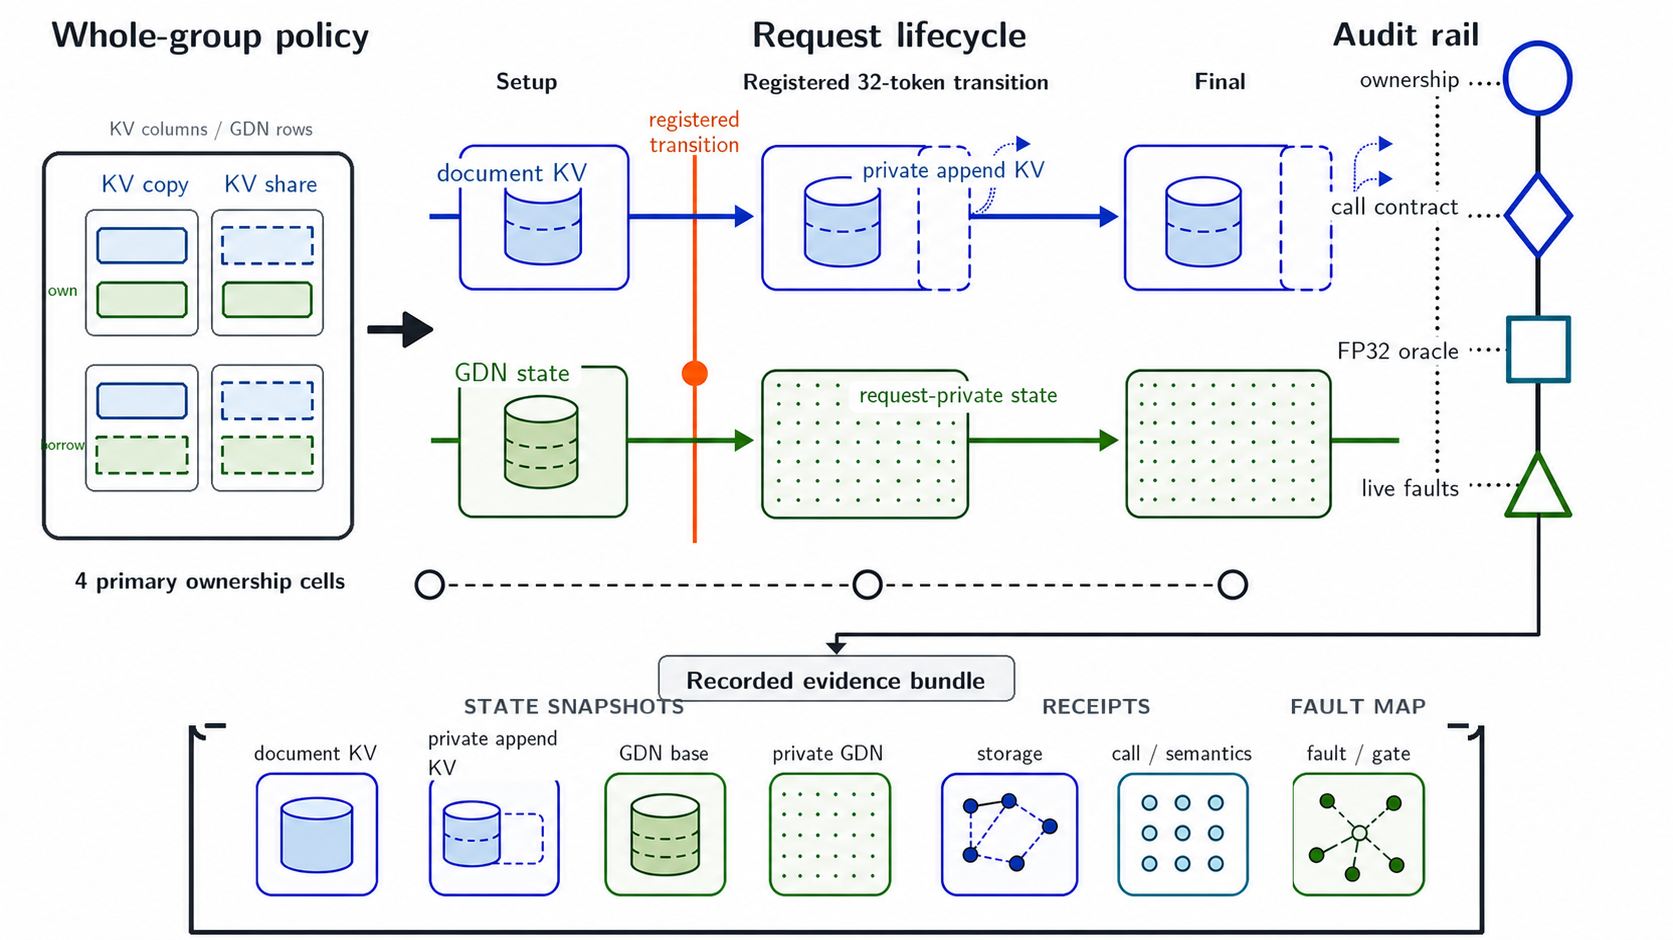
\includegraphics[width=0.98\textwidth]{figures/rr2_architecture_registered_transition.png}
  \caption{\method{} ownership factorial.  Four KV-by-GDN setup cells share
  immutable document state, keep append tails private, and rebind borrowed
  recurrent state at the registered transition.  The audit rail records
  lifecycle, storage, call/semantic, and fault-to-gate receipts.  This schematic
  details the validation component; it is not experimental evidence.}
  \label{fig:architecture}
\end{figure}

\begin{table}[H]
  \caption{Frozen primary-factorial execution geometry.  The eight ranks
  provide distinct books and query banks, not repeated stochastic
  measurements.}
  \label{tab:protocol}
  \centering
  \small
  \begin{tabular}{@{}p{0.25\linewidth}p{0.65\linewidth}@{}}
    \toprule
    Component & Frozen value \\
    \midrule
    Model & Qwen3.5-35B-A3B; 10 attention + 30 GDN layers \\
    Hardware & 8 $\times$ H20-3e; one book/rank \\
    Software & Python 3.11.13; PyTorch 2.11.0+cu129; Transformers 5.14.1; vLLM 0.26.0+cu129; Triton 3.6.0; CUDA 12.9 \\
    KV backend & vLLM fused attention; BF16; page 128 \\
    Document / query & 4,095 / 32 tokens; PG-19 train only \\
    Generation & 8 output tokens; 39 state-appended input tokens (32 query + 7 generated-token feedback) \\
    Resident counts & $1,8,32$; four KV-by-GDN ownership cells \\
    Primary schedule & all requests resident; batch-one sequential round-major calls on one CUDA stream/rank \\
    Validation & 96 factor configurations; separate memory/witness cells \\
    Fault campaigns & $N=2$; the primary all-gates-on campaign has nine live mutants with rebuilt controls; the target-gate-suppression campaign has nine fresh clean plus nine suppressed-gate cases on 8 H20s; the designer--executor-separated campaign has five new clean/mutant pairs on 5 H20s \\
    Historical regression & one previously encountered one-token alias defect; 8 ranks $\times$ 3 fresh $N=2$ lanes; 3 archived-coordinate reproductions + 5 additional frozen inputs; no mutation \\
    \bottomrule
  \end{tabular}
\end{table}

\begin{table}[H]
  \caption{Meaning of the live-binding rerun's selected-cell evidence units
  (archive entry \texttt{E-LIVE-BINDING-A}; Appendix~\ref{app:artifact}).
  Counts are per rank unless marked total; all belong to the same formal run.}
  \label{tab:v29-evidence-units}
  \centering
  \scriptsize
  \begin{tabular}{@{}p{0.21\linewidth}p{0.17\linewidth}p{0.54\linewidth}@{}}
    \toprule
    Unit & Count & Check and authorization \\
    \midrule
    Persistent sources & 60 & independently enumerated before the actual builder; exact object, storage, descriptor, and content remain fixed \\
    Selected anchors & 6/phase & preregistered persistent/request semantic rows; request-owned subset consumes the group-bound lineage capability \\
    Full live/serializer rows & 540/phase & $(1\text{ persistent}+8\text{ requests})\times60$ rows; live objects are re-enumerated and every serialized field, role, interval, content digest, and phase relation is checked \\
    Builder clone edges & 480 & $8\times60$ materialized destinations exhaust the captured persistent-rooted ledger and are direct \texttt{aten.clone} outputs \\
    Phase artifacts & 3 & setup, post-transition, and post-generation products are hash-bound, published to stable rank paths, and terminally reread \\
    Clean-memory context separation & 12 (96 total) & separate allocator-cell calls are all observed; zero selected-context overlaps mean the selected context did not enter them, not that the wrapper was absent or perturbation-free \\
    \bottomrule
  \end{tabular}
\end{table}

With field order (owner, request, layer, family, state), the six anchors are
$(\mathrm{Pers},\varnothing,0,\mathrm{rec},0)$,
$(\mathrm{Req},0,0,\mathrm{conv},0)$,
$(\mathrm{Req},0,1,\mathrm{conv},0)$,
$(\mathrm{Req},0,2,\mathrm{conv},0)$,
$(\mathrm{Req},0,2,\mathrm{rec},0)$, and
$(\mathrm{Req},1,0,\mathrm{rec},0)$.  The capability covers the five request
rows; the persistent row is their source anchor.

\begingroup
\footnotesize
\setlength{\LTpre}{0pt}
\setlength{\LTpost}{0pt}
\begin{longtable}{@{}>{\raggedright\arraybackslash}p{0.19\linewidth}>{\raggedright\arraybackslash}p{0.32\linewidth}>{\raggedright\arraybackslash}p{0.39\linewidth}@{}}
  \caption{Cohort-to-claim authorization.  Cohorts are never pooled; each row
  supports only the listed inference.}
  \label{tab:cohorts}\\
  \toprule
  Cohort & Frozen scope & Authorized claim / explicit exclusion \\
  \midrule
  \endfirsthead
  \multicolumn{3}{c}{\textit{Table~\ref{tab:cohorts} continued.}}\\
  \toprule
  Cohort & Frozen scope & Authorized claim / explicit exclusion \\
  \midrule
  \endhead
  \midrule
  \multicolumn{3}{r}{\textit{Continued on next page}}\\
  \endfoot
  \bottomrule
  \endlastfoot
  Primary ownership factorial & 8 books; PG-19; full-prefix BF16 KV; no split depth; no quantization; $N=1,8,32$; four KV$\times$GDN cells; 8 decode steps & ownership lifecycle, cross-cell equivalence, selected attention oracle, live-mutant sensitivity, and four-cell allocator endpoints; not the quantized Read path, and not transfer or scheduler evidence \\
  Primary target-5 rerun & same frozen 8-rank, 96-configuration Qwen/H20 factorial; 209,920 attention and 635,520 GDN calls & per-call selected Triton kernel-cache artifact/configuration and eager-route binding at the declared fixed-stack scope; not device-side completion, driver/device, compiled-GDN, ATen/CUDA, performance, or cross-stack evidence \\
  Selected-cell live binding & same frozen 8-rank factorial; stronger hook active only for the $N=8$ shared-document/materialized-GDN cell; actual builder, production serializer, and direct clone lineage & 144 selected rows, 12,960 live-storage rows, 3,840 clone edges, and 24 phase artifacts pass; all 96 clean-memory calls have zero selected-context overlaps; not evidence for other cells or coordinates, malicious runtimes, framework independence, device binaries, or performance \\
  Fresh-process control & one independent $N=2$ process; one clean path and M1 & input reconstruction, cleanup, and one intended-gate reproduction; not pooled with the factorial \\
  Lifecycle transfer & 8 books; aligned 4,096-token prefix; $N=4$; two cancelled slots & exact outputs/state, zero-scrub, exact reuse, and stale-lease rejection on the same adapter; not scheduler, concurrency, or performance evidence \\
  Scheduler interleave & 8 books; $N=4$; page/prefix/tail geometries 64/3,985/17 and 128/4,033/65; cancel slot 3 after round 2 & deterministic request-step interleaving, zero-scrub, epoch change, exact reuse, uninterrupted-control equality, and three frozen scheduler-fault gates; not concurrent kernels, continuous-batching performance, detection rate, or production end-to-end correctness \\
  Independent preproducer slot census & frozen Qwen/H20 geometry and schedule; 180 slots/capture; two $N=2$ GDN-policy cells and three phases/cell & all 6 captures, 1,080 receiver rows, and 96,660 relations close; omission, duplication, and semantic-relabel controls fail closed; producer manifests/rows are not expected-set authority, but slot-ID-to-live-tensor binding, IPC, and paused capture remain trusted \\
  Dual-producer repeat & same frozen input/protocol and producer implementation; two fresh serial executions and four distinct out-of-process observers & both executions reproduce 1,080 semantic coordinates, byte digests, stable descriptors, and 96,660 relation labels at zero tolerance; not malicious-producer resistance, independent receiver model execution, or cross-stack evidence \\
  Falcon-H1 bounded transfer & \path{tiiuae/Falcon-H1-0.5B-Base}; Transformers 5.14.1/H20 naive path; $N=1,2$; separately executed official Transformers reference; persistent-unquantized and deep-materialized arms & 8/8 ranks, 96 generated-token and 96 full-vocabulary FP32-logit comparisons, 13,824 state rows across KV key/value, convolution, and Mamba2 recurrent families, 192 ownership checks, cross-arm/cross-$N$ relations, and registered controls pass; no performance, memory, quality, or other-stack evidence \\
  Bounded two-stream lifecycle & one H20; one 4,033-token document; two 16-token query requests at $N=2$; two host threads and distinct CUDA streams; pre-cancel and post-reclaim phases; cancellation after synchronization & positive call-interval overlap plus exact four lifecycle outputs, 20 logical-KV layer pairs, two GDN slot aggregates, ownership, scrub, and reuse; not simultaneous kernels, native continuous batching, in-flight cancellation, production scheduling, or performance \\
  GDN transition oracle & 1 frozen book/window; global model-layer indices 0, 10, 20, 38; 4 query tokens & clean recurrence outputs/states and four seeded wrong-transition rejections conditional on post-normalization inputs; not all GDN layers or end-to-end semantics \\
  Expanded captured-boundary numerical sweep & 2 distinct PG-19 inputs; all 10 attention layers and 12 of 30 GDN layers; 20 attention and 24 GDN clean rows plus one seeded control/row & captured-boundary numerical agreement and rejection of all 44 seeded wrong operators; not upstream-activation, independent-capture, full-model, or end-to-end validation \\
  Target-gate suppression matrix & 9 fresh clean + 9 target-suppressed cases; same fixed model/data/$N=2$; 8 distinct H20s & per-fault comparison with redundant audit gates, exact allowlisted production assertions, and token/FP32-logit equality; M8's injected sentinel is not a detector; not a blind-fault study or rate \\
  Designer--executor-separated faults & separate designer reads only the prior PDF; 5 new frozen $N=2$ clean/mutant pairs; 5 H20s; all gates enabled & all 5 clean gates pass and all 5 mutants fail first at their frozen primary predicate; per-fault sensitivity only, not a detection rate, natural-defect study, or cross-stack evidence \\
  Historical alias regression & one pre-discovery integration defect; 3 archived coordinates + 5 additional frozen inputs; fresh pre-fix, repaired, and materialized $N=2$ one-token lanes; 8 H20s & pre-fix binding gate and base violation with output/terminal-state equality, plus storage-clean exact repair; one retrospective defect only, not prevalence, recall, statistical replication, or cross-stack evidence \\
  Mac common-mode control & Apple M4 Pro; six documents/queries; five fresh MLX processes; vanilla dense plus \qcomem{} BF16/Q8/Q4 at depth 7 & separates split-family agreement from agreement with vanilla dense; motivation only and separate from the H20 case \\
  H20 archival Store--F1 validation & 60 validation items from Qasper/2WikiMQA (30 each); dense, full-prefix, split, native dtype, frozen Q4/Q4/Q8, and two mixed policies & raw-first replay of Store, predictions, mean F1, paired bootstrap intervals, and fixed-case failure counts; not source-frozen regeneration, TTFT/TPOT/throughput, Recall, total memory, edge, or broad-benchmark evidence \\
  H20 operating-point run & the same 60 validation items; dense, full-prefix native dtype, full-prefix Q8, and \qcomem{} frozen Q4/Q4/Q8 at $j=13$ and $j=7$; one warm-up, three repeats, dataset-length generation, seed 20260903 & Store, TTFT, TPOT, mean F1, and paired bootstrap intervals against full-prefix from a separate execution; not pooled with the archival panel, not Recall, total memory, admitted capacity, resident-set, edge, or \method{} evidence \\
  H20 deployment timing & source indices 6--9 from each of Qasper/2WikiMQA (8 items total), a subset of the 60-item validation cohort; no-cache dense recompute, full-prefix KV reuse, and \qcomem{} Q8/Q4/mixed variants (six configurations total) with 3 timing repeats & same-stack retained-Store, TTFT, TPOT, tokens/s, and mean F1 comparison from a separate execution; not an independent replication, not pooled with the 60-item panel or primary factorial, and not scheduler/continuous-batching evidence \\
  Matched serving controls & 8 validation items from Qasper/2WikiMQA; vLLM 0.26 and SGLang 0.5.17 cache off/on plus 24 fixed-configuration HYPIC timing/quality cells; one H20-3e per item & within-block cache-hit, quality, and client-wall timing context; not pooled with in-process \qcomem{} timings, not a cross-framework leaderboard, and not continuous-batching evidence \\
  HYPIC retained-state receipts & 8 Prefix Cache + 8 HYPIC cells on the same fixed TP=1 model/slice; receipt-instrumented SGLang lifecycle & median target-entry-owned physical tensor payload only; not timing, NVML/process memory, capacity, continuous batching, or ForkAudit ownership evidence \\
  Related-work operator transfer & Hydragen at $N=8/32$ on one captured layer-3 attention family; Palu on one layer with 8 calibration and 1 held-out PG19 row & same-checkpoint numerical and logical-state trade-offs only; not an all-layer implementation, LongBench/quality result, speedup claim, or jointly optimized system \\
  Local replay/storage accounting & one Apple-silicon (M4-class) laptop CPU host; three consecutive fixed-order runs without cache flush; manifest-only core package plus a serial profile with five locally complete supporting verifiers & local CPU replay wall time and logical file/byte counts only; not H20 capture, GPU perturbation, cold-start latency, online inference, compressed-upload size, or an uninstrumented-baseline delta \\
\end{longtable}
\endgroup

\begin{table}[H]
\caption{The seven contract targets of Section~\ref{sec:contract}: trace
coverage, replay verdict, what a pass rules out, and the execution that
produced it.  A pass is trace-relative and conditional on capture honesty,
slot-to-live-tensor binding, and the target boundary of
Section~\ref{sec:contract}; it is not comprehensive system correctness.
Appendix Table~\ref{tab:witness} gives the decisive witness for each target.}
\label{tab:target-coverage}
\centering\scriptsize
\setlength{\tabcolsep}{3.2pt}
\begin{tabular}{@{}rlccp{0.33\linewidth}p{0.21\linewidth}@{}}
\toprule
\# & Target & Cov. & Verd. & A pass rules out & Execution; scope limit \\
\midrule
1 & Frozen identity & compl. & pass & a changed source, model, data, query, or protocol between capture and replay & primary rerun; one formal run \\
2 & Prefix immutability & compl. & pass & in-place writes to shared document KV or the GDN base at any phase & primary rerun; one frozen geometry \\
3 & Private ownership & compl. & pass & a request that still writes through an alias of the base or of a peer & primary rerun; live-binding rerun adds six owner-addressed rows per phase in one cell \\
4 & Tail-safe append & compl. & pass & a COW-elided in-place write to the partial final page & primary rerun; one partial-tail geometry \\
5 & Host-side launch/config. & compl. & pass & silent kernel fallback or route contamination on the host side & dispatch rerun; normal launcher return, not device completion \\
6 & Cross-arm equivalence & compl. & pass & an ownership arm that is cheaper because it computes something different & primary rerun; one sequential schedule \\
7 & Cross-$N$ consistency & compl. & pass & a prefix whose reuse depends on how many requests are resident & primary rerun; relational, not an independent oracle \\
\bottomrule
\end{tabular}
\end{table}


\begin{table}[H]
  \caption{Trace coverage and replay verdict for the seven contract targets in
  fresh frozen primary case.  Equality denotes canonical byte-digest identity
  as recorded.  Overall trace coverage is complete and all seven target
  verdicts pass at their declared fixed-stack scope.  A passing primary
  target verdict remains trace-relative and conditional on capture honesty,
  slot-ID-to-live-tensor binding, and the target boundary in Section~\ref{sec:contract}.
  The census removes producer rows as expected-set authority only for its bounded
  GDN cohort; supporting cohorts do not upgrade these targets to comprehensive
  system correctness.}
  \label{tab:witness}
  \centering
  \scriptsize
  \begin{tabular}{@{}>{\raggedright\arraybackslash}p{0.14\linewidth}p{0.11\linewidth}p{0.09\linewidth}>{\raggedright\arraybackslash}p{0.34\linewidth}>{\raggedright\arraybackslash}p{0.20\linewidth}@{}}
    \toprule
    Target & Trace coverage & Replay verdict & Decisive witness & Boundary \\
    \midrule
    Frozen identity & complete & pass & identical preflight/terminal source ledgers, terminal model rehash, and stable data/query/protocol/execution bindings & one primary-factorial formal run; the dual repeat recaptures only the bounded $N=2$ GDN cohort \\
    Prefix immutability & complete & pass & physical document-KV digests and GDN base guards across all three phases & one frozen configuration/geometry \\
    Private ownership & complete & pass & all-pairs request--base and request--peer range replay at the primary registered transition; actual-builder, serializer, and direct-clone receipts for the selected cell & pointer-free conservative intervals; stronger live binding covers only six selected rows per phase in one cell \\
    Tail-safe append & complete & pass & one-time 127-token private-tail copy before append & one partial-tail geometry \\
    Host-side launch/config. & complete & pass & per-call ID, selected kernel-cache artifact/configuration, autotuner outcome, GPU/stream, and post-return seal; source-bound GDN eager route & normal launcher return, not device completion; no driver/device, compiled-GDN, or ATen/CUDA attestation \\
    Cross-arm equivalence & complete & pass & tokens, shape/dtype-bound CPU-FP32 logit digests, logical KV, and GDN & one primary sequential schedule \\
    Cross-$N$ consistency & complete & pass & 288 all-arm adjacent-fan-out comparisons over 72 rank--query identities & relational, not an independent oracle \\
    \bottomrule
  \end{tabular}
\end{table}

Selected numerical oracles, constructed controls, lifecycle/scheduler checks,
the independent census and dual-producer repeat, bounded two-stream and Falcon
cohorts, and the historical reproduction are supporting checks rather than
additional contract targets.  Their captured-input, same-adapter,
process-separated-but-shared-IPC, second-configuration, and schedule boundaries
are reported separately.

\section{Pointer-Free Storage Witness Schema}
\label{app:storage-schema}

\paragraph{The pass predicate.}
For case specification \(\Sigma\), execution trace \(\tau\), mandatory slots
\(M_i(\Sigma)\), and replay predicates \(\Phi_i\),
\begin{equation}
  \operatorname{Pass}_i(\tau)\Longleftrightarrow
  [\operatorname{Coverage}_i(\tau)=\mathrm{complete}]
  \wedge\operatorname{Bind}_{\Sigma}(\tau)
  \wedge\bigwedge_{\phi\in\Phi_i}\phi(\tau),
\end{equation}
where completeness quantifies over \(M_i(\Sigma)\) --- every mandatory slot
present, unique, unmodified --- and \(\operatorname{Bind}_{\Sigma}\) requires
each slot to resolve to the live tensor its receipt names.  Coverage is therefore
separate from verdict: a missing, duplicated, modified, or unbound mandatory
receipt cannot silently pass.  The workflow freezes the run, captures
setup/transition/final digests, ranges, calls, semantics and allocator snapshots,
then replays every applicable predicate (Table~\ref{tab:normative-records}).

\paragraph{Target-to-record dependencies.}
The following matrix is normative.  I, L, E, and F denote the Identity,
Lifecycle, Execution, and Target/fault classes in Table~\ref{tab:normative-records};
parenthesized entries name mandatory fields.  Missing any marked field makes
that target open.  A preregistered geometry may make tail safety not applicable.
Target 5 additionally requires an exact per-call ID, selected kernel-cache
artifact/configuration, autotuner selection or explicit no-autotuner record,
assigned GPU/stream, and post-return seal; missing any applicable field leaves
target 5 open.  A missing F field invalidates the corresponding fault row,
but does not change the separately evaluated seven-target witness.

\paragraph{Enumerated evidence units and call counts.}
Section~\ref{sec:results} states the verdicts; the counts behind them are
collected here, each tagged with its execution.
\emph{Dispatch rerun.}  Host-side receipts for 209,920 attention calls record
the selected hashed Triton artifact/configuration and the
autotune/no-autotuner decision immediately before the original Python launcher,
then seal after normal return; another 635,520 receipts record the mutually
exclusive GDN eager route and functional cache rebind.  The totals factor as
$20{,}992\times10$ attention calls and $20{,}992\times30$ request-GDN calls plus
$192\times30$ one-time prefill calls.  They establish host-side selected
launch/configuration provenance only, not device-side operator identity,
execution, or completion, compiled GDN, underlying ATen/CUDA, or driver/device
binaries.
\emph{Live-binding rerun.}  Table~\ref{tab:v29-evidence-units} defines each
evidence unit.  The totals are $8\times3\times6=144$ selected-owner-row checks,
$8\times3\times540=12{,}960$ full serializer/live-object rows,
$8\times480=3{,}840$ direct clone edges, and $8\times3=24$ stable phase
artifacts, where the factor $3$ is the setup, post-transition, and
post-generation \emph{phases} --- not the three resident counts that appear in
the $8\times3\times4=96$ configuration product of
Section~\ref{sec:target-status}.  Here $60=30\times2$ persistent layer/family
coordinates (thirty GDN layers $\times$ recurrent and convolution families)
give the $480=8\times60$ direct clone destinations, and each phase contains the
full $540=(1+8)\times60$ serializer-row universe, one persistent plus eight
request owners, with six owner-row anchors.  All 96 separately enumerated
clean-memory calls occur outside the active selected context; zero
selected-context overlaps means only that this context never entered an
allocator cell, not that the wrapper was absent or perturbation-free.
\emph{Primary rerun.}  The 288 adjacent-fan-out comparisons of
Section~\ref{sec:results} span 72 rank--query identities across all arms, and
the borrowed-GDN arm's own allocator endpoints are $4.890\gib$ final and
$2.229\gib$ shared-document (Table~\ref{tab:rr2-memory}).  The primary
factorial's preregistered candidate-import-free NumPy oracle checks four GDN
transitions at global layer indices $0,10,20,38$ against four wrong
recurrences (Table~\ref{tab:gdn-oracle}), and its supporting cohorts derive
1,080 GDN observations and 96,660 relations from a source-distinct
expected-slot census (Appendix~\ref{app:controls}).

\begin{center}
\scriptsize
\setlength{\tabcolsep}{2.5pt}
\begin{tabular}{@{}p{0.13\linewidth}p{0.17\linewidth}p{0.17\linewidth}p{0.20\linewidth}p{0.08\linewidth}p{0.14\linewidth}@{}}
\toprule
Target & I & L & E & F & Blind predicate \\
\midrule
Frozen identity & code, model, data, protocol; role map & --- & --- & N/A & exact bytes and complete roles \\
Prefix immutability & document/base roles; start digests & setup and final guards & canonical content digests & N/A & start $=$ final \\
Private ownership & request/base/private roles & setup, registered-transition, final bindings & normalized storage ranges & N/A & non-vacuous all-pairs disjointness \\
Tail-safe append & page geometry; document/private roles & first append event & ordered append and copied-tail receipt & N/A & one private copy before write \\
Host-side launch/config. & callable, source, protocol, selected artifact/config. & post-return seal; GPU/stream assignment & ordered call, query, mask, position, append, scale, autotuner outcome, eager route & N/A & exact per-call binding; no fallback or route contamination \\
Cross-arm equivalence & factor, query, and schedule identities & final bindings & token, logit, logical-KV, GDN records & N/A & canonical semantic equality \\
Cross-$N$ consistency & query and fan-out identities & --- & the same canonical semantic records & N/A & smallest-$N$ equals each larger $N$ \\
Fault sensitivity (supporting) & frozen target/gate map & matched-control rebuild and cleanup & injected outcome and failed predicates & required & target, injection, expected gate, outcome \\
\bottomrule
\end{tabular}
\end{center}

Each tensor-view row has the exact fields
\texttt{storage\_id}, \texttt{shape}, \texttt{stride},
\texttt{storage\_offset}, \texttt{dtype}, \texttt{device},
\texttt{storage\_nbytes}, \texttt{tensor\_nbytes}, and
\texttt{content\_sha256}; absolute addresses are forbidden.  Within each
phase, the producer assigns \texttt{storage-0000}, \texttt{storage-0001},
and so on in first-observation order to backing storages.  Reusing an ID with
a different device or storage size is invalid.  Phase capture IDs are unique,
whereas request and persistent lifecycle-guard IDs must remain stable across
setup, the registered transition, and final generation.

Let element size be $e$, storage offset $o$, shape $s_i$, and stride $t_i$.
The independent replay initializes $m=M=o$ and, for every dimension, computes
\begin{equation}
  d_i=(s_i-1)t_i,\qquad
  m\mathrel{+}=\min(d_i,0),\qquad
  M\mathrel{+}=\max(d_i,0).
\end{equation}
The conservative half-open byte interval is
\begin{equation}
  I=[em,\,e(M+1)),
\end{equation}
which must be non-negative and contained in \texttt{storage\_nbytes}; also
\texttt{tensor\_nbytes}$=e\prod_i s_i$.  Two rows overlap iff their normalized
storage IDs match and $I_a^{\mathrm{start}}<I_b^{\mathrm{end}}$ and
$I_b^{\mathrm{start}}<I_a^{\mathrm{end}}$.  Exact aliasing additionally
requires equality of interval, geometry, dtype/device, storage and tensor
sizes, and content digest.  For correctly live-bound rows at one capture, if
represented views sharing physical backing receive the same normalized ID and
their shape, stride, offset, and element size exactly describe affine-strided
views, $I$ contains every touched byte.  The overlap test then cannot miss a
shared byte between represented rows, although interleaving may cause false
positives.  Omitted rows, between-capture changes, and wrapper or storage-ID
violations remain outside the claim.

At setup, every recurrent-state coordinate must either exactly alias the
persistent state (borrowed-base arm) or be disjoint from it (materialized
arm).  At the primary registered 32-token transition boundary, a completed
request's 60 mutable rows must be disjoint from the base and every peer;
incomplete borrowed requests must
remain exact aliases.  At final, all request-local GDN states must be disjoint
from the persistent GDN base and every peer; document KV remains intentionally
shared.
Independent binding-token receipts additionally require unchanged tokens for
incomplete requests and changed binding/storage tokens for completed requests.
The package applies this schema to all 96 timelines and 288 phase artifacts;
nine adversarial tests cover exact aliasing, partial overlap, adjacent
intervals, negative strides, conflicting ID reuse, pointer injection,
capture/guard reuse, and cross-coordinate request--base and request--peer
aliasing.

\section{Executed Fault Rows and Invariant Map}
\label{app:invariants}

The row-level campaign is kept out of the main paper because it supports
diagnosis and audit coverage rather than a separate headline result.
Separately, the CPU governance suite passes 17 tests and rejects 28 explicit
serialized-artifact tamper cases plus its registered helper/launcher faults.
That result concerns schema and orchestration fail-closure only; it is not GPU
semantic or performance evidence.
\begin{table}[H]
\caption{Separate primary all-gates-on reference. Every separately rebuilt matched-clean cell passed; every mutant reached its target gate fixed before execution and was restored before disposal.}
\label{tab:rr2-mutants}
\centering\footnotesize
\begin{tabular}{@{}clll@{}}
\toprule
ID & Injected live fault & Expected/observed gate & Primary outcome \\
\midrule
M1 & reservation alias & \texttt{KV\_RESERVATION\_DISJOINT} & target gate reached \\ 
M2 & sequence swap & \texttt{KV\_SEQUENCE\_ID} & target gate reached \\ 
M3 & omit tail COW & \texttt{KV\_TAIL\_COW} & target gate reached \\ 
M4 & GDN--base alias & \texttt{gdn\_completed\_vs\_base\_disjoint} & target gate reached \\ 
M5 & GDN peer alias & \texttt{gdn\_completed\_vs\_peers\_disjoint} & target gate reached \\ 
M6 & position off-by-one & \texttt{POSITION\_CANONICAL\_VALUES} & target gate reached \\ 
M7 & materialized mask & \texttt{MASK\_CONTRACT} & target gate reached \\ 
M8 & wrong callable & \texttt{KERNEL\_CALLABLE\_ID} & target gate reached \\ 
M9 & dense KV view & \texttt{KV\_PAGED\_VIEW} & target gate reached \\ 
\bottomrule
\end{tabular}
\end{table}


\begin{table}[H]
\caption{Same-system outcomes for nine designed faults.  The primary campaign
enables all gates; a separate target-gate-suppression campaign suppresses only
the named gate.
``Same'' is exact and ``N/O'' an earlier stop.  Rows are not a detection rate;
M8's injected sentinel is not a production detector.}
\label{tab:first-gate-localization}
\centering\scriptsize
\setlength{\tabcolsep}{2.6pt}
\begin{tabular}{@{}p{0.19\linewidth}p{0.12\linewidth}p{0.39\linewidth}p{0.18\linewidth}@{}}
\toprule
Fault / target contract & All gates on & With target gate suppressed & Token / FP32 logits \\
\midrule
M1 Reservation ownership & target gate & completes & Same / Same \\
M2 Sequence binding & target gate & completes & Same / Same \\
M3 Tail COW & target gate & other audit: active-block ownership & N/O / N/O \\
M4 GDN base isolation & target gate & other audit: peer isolation & N/O / N/O \\
M5 GDN peer isolation & target gate & completes; logits change ($L_\infty=0.75$, rel. $L_2=0.0314$) & Same / Changed \\
M6 Positions & target gate & completes & Same / Same \\
M7 Mask contract & target gate & completes & Same / Same \\
M8 Callable identity & target gate & injected payload sentinel & N/O / N/O \\
M9 Paged-KV view & target gate & paired-view production assertion & N/O / N/O \\
\bottomrule
\end{tabular}
\end{table}


\paragraph{Designer--executor-separated fault detail.}
The five fixed per-fault outcomes summarized in the main text are shown below;
they remain constructed controls rather than a defect-population sample.
\begin{table}[H]
\caption{Designer--executor-separated constructed fault outcomes.  A separate
designer saw only a frozen earlier manuscript PDF and fixed all five
definitions, loci, payloads, clean requirements, and expected first predicates
before executor preparation or candidate output.  The cases are separated from
executor preparation and outcome inspection, not from the predicate vocabulary.  All
matched clean cases pass; every mutant completes its
registered horizon and is rejected first by the frozen primary predicate.
Semantic comparisons are secondary: ``Same'' means canonical exact equality
with the matched clean case, KV/GDN denote terminal logical state, and ``N/C''
means full-logit call cardinality is not comparable.  These five fixed outcomes
are not a population detection rate.}
\label{tab:r33-fresh-heldout}
\centering\scriptsize
\setlength{\tabcolsep}{2.5pt}
\begin{tabular}{@{}p{0.18\linewidth}p{0.22\linewidth}p{0.27\linewidth}p{0.22\linewidth}@{}}
\toprule
Frozen fault & Isolated mutation & First failed predicate & Tokens / logits / KV / GDN \\
\midrule
HF01 delayed tail detach & append write precedes the otherwise present tail copy & tail-copy-before-first-write & Same / Same / Same / Same \\
HF02 inactive-lane scribble & one bit in the unused lane of a shared physical K page & physical-prefix immutability & Same / Same / Same / Same \\
HF03 duplicate commit & one correct feedback call commits twice; first output discarded & ordered-call cardinality & Same / N/C / Changed / Changed \\
HF04 effective-scale drift & first registered attention scale is exactly doubled & attention effective scale & Changed / Changed / Changed / Changed \\
HF05 stale GDN binding token & storage correctly rebinds; lifecycle token remains stale & completed binding-token advance & Same / Same / Same / Same \\
\bottomrule
\end{tabular}
\end{table}


\begin{table}[H]
\caption{Representative failure families and intended checks.  Rows naming
M1--M9 refer to the nine executed primary-factorial live mutants; the other
rows summarize schema, relational, numerical, or replay checks.  None is a
complete oracle.}
\centering\small
\begin{tabular}{@{}p{0.23\linewidth}p{0.66\linewidth}@{}}
\toprule
Check family & Intended sensitivity and observed boundary \\
\midrule
Frozen identity & wrong model/data/query bank, changed protocol, stale shard (schema adversaries)\\
Prefix immutability & M3 omits partial-tail COW; physical document digest and ownership gates fail\\
Private ownership & M1 reservation alias, M4 request--base GDN alias, M5 request--peer GDN alias\\
Sequence/view binding & M2 sequence swap and M9 dense-KV replacement\\
Host-side selected launch/configuration & M6 position offset, M7 materialized mask, M8 wrong callable\\
Factorial exactness & behavior changes when either KV or GDN setup ownership changes\\
Bounded numerical oracle & numerical error in a selected fused full-attention result\\
Raw replay & internally inconsistent trajectory, storage, allocator, or aggregate fields\\
\bottomrule
\end{tabular}
\end{table}

The primary all-gates-on execution is a first-gate localization study. Every
registered gate fires before the injected path produces a post-injection
token, logit, logical-KV digest, or GDN digest; its output cells are therefore
N/O rather than misses. Lifecycle/ownership/storage receipts supply the first
gate for M1 and M3--M5; request-binding/call receipts supply it for M2 and
M6--M9. The full audit rejects all nine at their predeclared gates under
passing matched controls. The separate target-gate-suppression matrix then
suppresses one named gate per mutant while leaving the remaining observers
active. It provides the per-fault comparison in
Table~\ref{tab:first-gate-localization}, but does not estimate a population
rate, unseen-fault coverage, or false-positive rate.

\section{Relation to Prior Work and Audit Obligations}
\label{app:novelty-boundary}

This appendix carries the attributions and distinctions Section~\ref{sec:related}
points to.

\paragraph{The established quantization surfaces.}
KIVI, KVQuant and XQuant fix the grouping axis or the tensor
quantized~\citep{liu2024kivi,hooper2024kvquant,tomar2025xquant}; KVTuner and
AsymKV assign layer-wise mixed-precision KV bit pairs
offline~\citep{li2025kvtuner,tao2025asymkv,yang2024mikv}; Palu, SqueezeAttention
and HeadKV allocate rank or budget rather than
bits~\citep{chang2025palu,wang2025squeezeattention,fu2025headkv}; and Quamba,
Quamba2 and MambaQuant quantize selective-SSM activations and per-state-group
recurrent inputs, including for a hybrid
backbone~\citep{chiang2025quamba,chiang2025quamba2,yue2025mambaquant}.  Our bit
vector $\mathbf b$ is one setting on this surface, not a new selection method.

\paragraph{The two differences from XQuant.}
The cut point is a depth-$j$ boundary residual, not a layer
input~\citep{tomar2025xquant}, so what is recomputed is the whole suffix $[j,L)$
for a later query over a persisted document, not one layer's projections inside
its own decode step.  And the retained object is not one family: below the split
a hybrid backbone still needs full-attention KV with convolution and recurrent
state its kernels mutate in place, so the entry is heterogeneous and raises the
ownership question of Section~\ref{sec:read} that a dense activation cache does
not.

\paragraph{Evaluation-methodology precedents.}
SCBench emphasizes cache lifecycles~\citep{li2025scbench}; metamorphic testing,
MT-DLComp, and CRADLE motivate preserved relations and independent
checks~\citep{chen2018metamorphic,xiao2022metamorphic,pham2019cradle}; DNNMem
separates memory denominators~\citep{gao2020dnnmem}.

\begin{table}[H]
  \caption{Primary-source positioning.  ``Evidence focus'' describes what the
  cited work evaluates; it is not a claim that the work lacks all other checks.}
  \label{tab:closest}
  \centering
  \footnotesize
  \begin{tabular}{@{}p{0.16\linewidth}p{0.28\linewidth}p{0.43\linewidth}@{}}
    \toprule
    Work & Primary mechanism & Evidence focus / relation to this work \\
    \midrule
    PagedAttention & Paged KV allocation and sharing~\citep{kwon2023pagedattention} & Serving throughput and memory utilization; supplies the block-sharing substrate. \\
    SGLang / Prompt Cache & Prefix reuse in structured or modular prompts~\citep{zheng2024sglang,gim2024promptcache} & Runtime performance and output behavior; establish reuse and positional handling as prior art. \\
    CoMem & One persistent residual per token at split $j$; bounded selection; suffix replay~\citep{liu2026comem,liu2026understanding} & Supplies the split-replay foundation; we do not claim that primitive as new. \\
    XQuant & Quantized layer-input activation cache with key/value rematerialization at decode~\citep{tomar2025xquant} & Closest prior art on the quantize-an-intermediate-and-recompute idea, which we therefore do not claim; it cuts inside a layer on a dense backbone, whereas we cut at a depth-$j$ boundary and retain heterogeneous lower attention KV plus mutable convolution/recurrent state. No head-to-head comparison is reported. \\
    \qcomem{} (ours) & Joint low-bit split residual and required lower KV/convolution/recurrent state & Adds complete hybrid-state packing, a capacity--latency--quality evaluation, and an auditable request-local ownership boundary; not a model-weight compressor or production scheduler. \\
    Marconi & Admission and eviction for hybrid-model prefixes~\citep{pan2025marconi} & Hybrid cache hit rate and time to first token; closest state-heterogeneous caching system, but a different policy-level contribution. \\
    SCBench & Lifecycle-oriented KV-cache benchmark~\citep{li2025scbench} & Breadth over tasks and cache phases; exposes breadth absent from our bounded declared configurations. \\
    MT-DLComp / CRADLE & Metamorphic compiler testing and cross-backend differential checking~\citep{xiao2022metamorphic,pham2019cradle} & Direct testing precedents; our audit adds ownership witnesses and a layerwise dense oracle, but not an independent end-to-end backend. \\
    DNNMem & Component-wise GPU-memory accounting~\citep{gao2020dnnmem} & Supports denominator separation; it is an estimator, not a request-ownership audit. \\
    \method{} & Typed, phase-indexed ownership/call/accounting trace with explicit coverage semantics & Validates the ownership component through a mutation-tested KV-by-GDN factorial, bounded host-side call receipts, a preproducer expected-slot census, numerical sweeps, and one bounded Falcon-H1 comparison; it is not a security attestation or general end-to-end correctness oracle. \\
    \bottomrule
  \end{tabular}
\end{table}

\begin{table}[H]
\caption{Closest established precedent for each audit obligation.  The final
column states the narrower integration contributed by \method{}; it does not
claim that any individual mechanism is new.}
\centering\scriptsize
\begin{tabular}{@{}p{0.18\linewidth}p{0.31\linewidth}p{0.42\linewidth}@{}}
\toprule
Audit obligation & Closest established precedent & Integrated obligation in this work \\
\midrule
Frozen identity & Controlled variants in metamorphic and differential testing~\citep{chen2018metamorphic,xiao2022metamorphic,pham2019cradle} & Bind model, data, query bank, callable contract, and protocol bytes to every ownership receipt. \\
Document immutability and tail COW & PagedAttention block sharing and copy-on-write for shared prefixes~\citep{kwon2023pagedattention} & Replay physical document pages, padding, active tables, and the partial-tail detach event. \\
Recurrent-state ownership & Hybrid recurrent states and their in-place update constraint~\citep{yang2025gateddeltanet,pan2025marconi} & Witness request--base and request--peer ranges before and after the frozen schedule's registered transition boundary. \\
Host-side selected launch/configuration & Cross-backend differential checking exposes implementation-dependent behavior~\citep{pham2019cradle} & Hold the backend fixed; record callable, positions, mask, scale, and append history; and bind the selected Triton kernel-cache artifact/configuration per attention call while keeping GDN at an explicit eager-route boundary. \\
Cross-arm and cross-$N$ relations & Metamorphic relations over semantics-preserving transformations~\citep{chen2018metamorphic,xiao2022metamorphic} & Treat ownership policy and resident fan-out as transformations that must preserve registered request observables. \\
Bounded numerical oracle & Independent backend comparison~\citep{pham2019cradle} & Reconstruct selected attention inputs for dense IEEE-FP32 math and selected post-normalization GDN inputs for a candidate-import-free NumPy recurrence. \\
Memory denominators & Component-wise GPU-memory accounting~\citep{gao2020dnnmem} & Keep page geometry, allocator current/peak, and unmeasured process/service capacity as separate claim domains. \\
\bottomrule
\end{tabular}
\end{table}

\FloatBarrier

\section{Supporting Control Experiments}
\label{app:controls}

\paragraph{Mac common-mode motivation.}
The archival Apple-M4-Pro control is kept unpooled from the H20 experiments and
serves only to show why split-family agreement does not replace a dense or
independently implemented oracle.
\begin{table}[H]
\caption{Unpooled Mac motivation context (Apple M4 Pro, five fresh MLX processes; median over 30 query executions at split depth 7). Vanilla dense is the external reference. \qcomem{} BF16/Q8/Q4 variants use the same selected documents. Store size is the six-document residual corpus; online time includes query Write, dequantization, and suffix Read. This small teacher-forced demonstration set is not primary ForkAudit evidence and supports no cross-hardware or production-speed claim.}
\label{tab:mac-motivation}
\centering\scriptsize
\setlength{\tabcolsep}{2.7pt}
\begin{tabular}{@{}lrrrr@{}}
\toprule
Method & Store (MiB) & Online (ms) & Speedup & Top-1 vs. dense \\
\midrule
Vanilla dense prompt & -- & 194.70 & 1.00$\times$ & 100.00\% \\
\qcomem{} BF16 split & 1.998 & 168.88 & 1.15$\times$ & 71.89\% \\
\qcomem{} Q8 split & 1.061 & 169.17 & 1.15$\times$ & 71.89\% \\
\qcomem{} Q4 split & 0.562 & 169.25 & 1.15$\times$ & 71.89\% \\
\bottomrule
\end{tabular}
\vspace{0.5mm}
\parbox{0.98\linewidth}{\scriptsize Q8/Q4 retain 100\% top-1 agreement with the BF16 split path, yet all split rows inherit only 71.89\% agreement with vanilla dense. The speed column is a small teacher-forced mechanism benchmark, not production RAG throughput.}
\end{table}


\paragraph{Historical alias regression and repair.}
The pre-fix, repaired, and materialized lanes isolate one previously observed
recurrent-state alias.  This is a fixed mechanism study, not a natural-bug
frequency or detector-recall estimate.
\begin{table}[H]
\caption{Retrospective reproduction and repair of one historical alias
regression.  Ranks 0--2 reuse three archived input coordinates; ranks 3--7
are additional frozen inputs, not additional defects or statistical
replicates.  Semantic columns compare each path with a fresh materialized
control.  ``Base inv.'' is within-path persistent-base immutability, retained
as a conventional state-invariant catch.}
\label{tab:r35-historical-alias}
\centering\scriptsize
\setlength{\tabcolsep}{2.1pt}
\begin{tabular}{@{}>{\raggedright\arraybackslash}p{0.14\linewidth}>{\raggedright\arraybackslash}p{0.08\linewidth}>{\raggedright\arraybackslash}p{0.20\linewidth}p{0.075\linewidth}p{0.085\linewidth}p{0.09\linewidth}p{0.075\linewidth}p{0.07\linewidth}@{}}
\toprule
Coordinates & Path & Ownership result & Token & FP32 logits & Request GDN & Logical KV & Base inv. \\
\midrule
Archived (3) & Pre-fix & binding gate 3/3 & exact 3/3 & exact 3/3 & exact 3/3 & exact 3/3 & fail 3/3 \\
Archived (3) & Repaired & storage-clean 3/3 & exact 3/3 & exact 3/3 & exact 3/3 & exact 3/3 & pass 3/3 \\
Additional (5) & Pre-fix & binding gate 5/5 & exact 5/5 & exact 5/5 & exact 5/5 & exact 5/5 & fail 5/5 \\
Additional (5) & Repaired & storage-clean 5/5 & exact 5/5 & exact 5/5 & exact 5/5 & exact 5/5 & pass 5/5 \\
\bottomrule
\end{tabular}
\end{table}


\paragraph{Primary allocator endpoints and fixed-case detection detail.}
Token equality catches $0$ of $5$ semantics-completing mutants and exact logits
$1$ of $5$ (Table~\ref{tab:first-gate-localization}); in the no-injection
defect, output and terminal request state stay exact in 8/8 cells under
persistent-base corruption that Table~\ref{tab:r35-historical-alias}'s invariant
also catches on all eight pre-fix cells.  The four ownership cells below use one
frozen post-priming allocator denominator and are kept separate from deployment
Store.
Against the appropriate reference the ownership component saves nothing:
Table~\ref{tab:rr2-memory}'s paged-prefix baseline is the closest same-stack
system, and at $N=32$ our audited fork ties it exactly ($2.229\gib$ final,
$2.843\gib$ peak) while being $1.950$ against $0.019\gib$ worse on generation
increment, so the design buys auditable request-local state, not fewer allocator
bytes.  The $54.5\%$/$42.2\%$ figures are measured against a different arm: with
materialized GDN setup, shared-document rather than full-copy KV cuts the final allocated
delta from $4.901$ to $2.229\gib$ ($54.5\%$) and the peak from $4.920$ to
$2.843\gib$ ($42.2\%$) above the frozen post-priming baseline.  That full-copy
arm is a controlled ownership factor, not an optimized baseline: no serving
engine copies a shared prefix per request, and the saving is block
sharing~\citep{kwon2023pagedattention}.
\begin{table}[H]
\caption{Primary 8$\times$H20-3e allocator results at $N=32$ (median across ranks; rank values coincide). Full-copy is the factorial control; the paged-prefix row is the closest same-stack prefix-sharing baseline. The remaining rows isolate recurrent-base ownership. All cells retain the persistent document source. Values are GiB above the frozen post-priming baseline; generation increment is the additional peak above allocation present at generation start.}
\label{tab:rr2-memory}
\centering\scriptsize
\setlength{\tabcolsep}{2.6pt}
\begin{tabular}{@{}p{0.25\linewidth}p{0.25\linewidth}rrr@{}}
\toprule
Empirical arm & KV / GDN setup & Final & Peak & Gen. incr. \\
\midrule
Full-copy factorial control & Full-copy KV / Materialized GDN base & 4.901 & 4.920 & 0.019 \\
GDN ownership ablation & Full-copy KV / Borrowed GDN base & 4.890 & 4.907 & 1.951 \\
Paged-prefix baseline & Shared-doc KV / Materialized GDN base & 2.229 & 2.843 & 0.019 \\
Audited hybrid fork & Shared-doc KV / Borrowed GDN base & 2.229 & 2.843 & 1.950 \\
\bottomrule
\end{tabular}
\end{table}


\paragraph{Published systems context.}
Table~\ref{tab:published-context} reports each cited system only in its native
protocol and keeps all non-commensurate metrics outside our matched panels.
This unpooled table is literature context, not ForkAudit evidence.
\begin{table}[H]
\caption{Unpooled published-systems context in each paper's native protocol.  These values show the scale and evaluation breadth of related systems, \emph{not} a cross-paper leaderboard or ForkAudit evidence: models, hardware, batching, baselines, and metrics differ.  Consequently, no row is merged with our same-stack H20 Table~\ref{tab:h20-deployment}, and the absence of a common score must not be read as a negative result.}
\label{tab:published-context}
\centering\scriptsize
\setlength{\tabcolsep}{2.5pt}
\begin{tabular}{@{}>{\raggedright\arraybackslash}p{0.15\textwidth}>{\raggedright\arraybackslash}p{0.28\textwidth}>{\raggedright\arraybackslash}p{0.265\textwidth}>{\raggedright\arraybackslash}p{0.245\textwidth}@{}}
\toprule
System & Native method and study setting & Reported efficiency in its native protocol & Quality and comparability boundary \\
\midrule
PagedAttention / vLLM~\citep{kwon2023pagedattention} & Paged KV allocation plus serving engine\newline \textit{Setting:} LLaMA-7B on A10G and LLaMA-13B on A100-40GB; vLLM serving engine & 2--4$\times$ serving throughput at similar latency vs. FasterTransformer/Orca & No common LongBench F1; exact cache-management method \\
Prompt Cache~\citep{gim2024promptcache} & Modular attention-state reuse\newline \textit{Setting:} Llama2/MPT/Falcon; RTX 4090, A40, and A100; HuggingFace-style prototype & 1.5--3.1$\times$ TTFT (CPU-resident modules); 3.7--11.7$\times$ (GPU-resident) on its 12-dataset LongBench suite & LongBench accuracy evaluated, but with different models and hardware \\
SGLang / RadixAttention~\citep{zheng2024sglang} & Prefix reuse plus structured-program runtime\newline \textit{Setting:} Llama-7B/Mixtral-8x7B and structured programs; A10G/A100; SGLang & Up to 6.4$\times$ throughput vs. prior inference systems & Application-suite result; no common LongBench F1 \\
ChunkAttention~\citep{ye2024chunkattention} & Prefix-aware KV chunks and attention kernel\newline \textit{Setting:} attention microbenchmarks; mainly A100-80GB, plus A100-40GB/RTX 4090; CUDA 11.8 & 3.2--4.8$\times$ attention-kernel speedup for 1K--4K shared prompts & Kernel result; no end-to-end common task score \\
Hydragen~\citep{juravsky2024hydragen} & Exact batched shared-prefix attention\newline \textit{Setting:} CodeLlama-13B/34B shared-prefix batches; A100 (with H100/L40S microbenchmarks); custom HuggingFace runtime & Up to 32$\times$ CodeLlama-13B end-to-end throughput in large shared-prefix batches & Exact attention construction; different model and batching regime \\
Palu~\citep{chang2025palu} & Low-rank latent KV with reconstruction/fusion\newline \textit{Setting:} Llama/Mistral/LongChat quality studies; Llama-2-7B latency on one RTX 4090; HuggingFace plus custom kernels & 50\% KV compression and up to 1.89$\times$ RoPE-attention speedup; up to 2.91$\times$ with quantization & Llama/Mistral/LongChat native study; our bounded Qwen3.5 operator transfer is reported separately \\
Preble~\citep{srivatsa2025preble} & Distributed prompt-sharing scheduling\newline \textit{Setting:} Mistral-7B/Llama-3-70B request traces; two--eight GPUs across A6000/H100 clusters; distributed serving & 1.5--14.5$\times$ average-latency and 2--10$\times$ p99-latency improvement & Distributed serving traces; no common task score \\
Marconi~\citep{pan2025marconi} & Admission/eviction for hybrid-model prefixes\newline \textit{Setting:} Attention--Mamba2 7B geometry; LMSys/ShareGPT/SWE-bench traces; CloudLab policy simulation & Up to 34.4$\times$ token-hit rate and up to 71.1\% or 617 ms lower TTFT & Hybrid models and trace-driven policy study; no common LongBench F1 \\
KVTuner~\citep{li2025kvtuner} & Offline sensitivity-aware search over layer-wise mixed-precision KV bit pairs\newline \textit{Setting:} Llama-3.1-8B-Instruct and Qwen2.5-7B-Instruct; mathematical- and general-reasoning suites & Nearly lossless 3.25-bit mixed-precision KV for Llama-3.1-8B-Instruct and 4.0-bit for Qwen2.5-7B-Instruct; up to 21.25\% higher maximum inference throughput vs. KIVI-KV8 & Layer-wise bit search for a dense KV cache; it does not quantize a split residual or recurrent state, and no common Qwen3.5 slice exists \\
HYPIC~\citep{liu2026hypic} & Position-independent caching for hybrid full/linear-attention models\newline \textit{Setting:} Qwen3.5-35B-A3B main panels at TP=2 on 8 H20-3e; SGLang 0.5.14 & 3.25$\times$ lower TTFT on average and 1.66$\times$ higher QPS over Prefix Cache & Four models/five workloads; our same-slice TP=1 timing and retained-state controls are reported separately \\
\bottomrule
\end{tabular}
\end{table}


\paragraph{Same-checkpoint transfer detail.}
Table~\ref{tab:related-transfer} is the matched complement to the published
context table: it uses our frozen Qwen3.5 checkpoint and H20-3e, binds the
official Hydragen and Palu source revisions, and independently replays all raw
operator sidecars.  Because it does not execute all layers or LongBench, it is
kept separate from Table~\ref{tab:h20-deployment}.
\begin{table}[H]
\caption{Bounded same-checkpoint H20 transfers.  Hydragen uses frozen Qwen3.5
layer-3 post-RoPE attention; Palu uses eight 256-token PG19 calibration rows
and one disjoint held-out row.  Errors are relative $\ell_2$ against the
matched uncompressed operator; state ratios are logical selected-operator
ratios, not process memory or end-to-end results.}
\label{tab:related-transfer}
\centering\scriptsize
\setlength{\tabcolsep}{2.8pt}
\begin{tabular}{@{}p{0.16\linewidth}p{0.12\linewidth}p{0.25\linewidth}p{0.20\linewidth}p{0.18\linewidth}@{}}
\toprule
Port & Setting & Matched numerical result & Logical state result & Timing / boundary \\
\midrule
Hydragen port & $N=8$ & Hydragen--dense rel. $\ell_2=0.00255$ & 8.50 vs. 64.48 MiB ($7.59\times$ smaller) & 0.287 vs. 0.0965 ms; no speedup \\
Hydragen port & $N=32$ & Hydragen--dense rel. $\ell_2=0.00262$ & 10.00 vs. 257.94 MiB ($25.80\times$ smaller) & 0.290 vs. 0.259 ms; no speedup \\
\midrule
Palu port & rank 64/head & held-out K/V $0.487/0.549$ (plain $0.711/0.839$) & 512 vs. 2,048 B/token ($4.00\times$ smaller) & projection only; no fused kernel \\
Palu port & rank 128/head & held-out K/V $0.317/0.364$ (plain $0.543/0.668$) & 1,024 vs. 2,048 B/token ($2.00\times$ smaller) & projection only; no fused kernel \\
Palu port & rank 192/head & held-out K/V $0.149/0.194$ (plain $0.341/0.459$) & 1,536 vs. 2,048 B/token ($1.33\times$ smaller) & projection only; no fused kernel \\
\bottomrule
\end{tabular}
\vspace{0.5mm}
\parbox{0.97\textwidth}{\footnotesize Hydragen avoids prefix replication but
has no speedup here.  Palu improves over plain SVD, but residual error forbids
an end-to-end quality claim.  Neither is a jointly optimized combined system.}
\end{table}


\subsection{Extended Deployment and Serving Context}
\label{app:illustrative-store}

Table~\ref{tab:qcomem-tradeoff}a is the matched Transformers block behind the
latency result of Section~\ref{sec:latency} and is printed in the body; the
expanded table below repeats that block to place separately measured
SGLang/HYPIC context beside it, and inherits panel~(a)'s reporting caveats,
including a throughput column that reconciles with no generated-token count.
The blocks use different runtimes and harnesses, so timing and F1 are
interpreted within block and are not pooled.  These serving controls are not
\method{} validation evidence and do not establish robust quality preservation.

\begin{table}[!ht]
\caption{Illustrative same-checkpoint H20 retained Store and mean-F1 point
estimates on an eight-item Qasper/2WikiMQA slice.  All rows use
Qwen3.5-35B-A3B, one H20-3e per item, a 4,096-token cap, greedy decoding, and
at most 32 generated tokens.  The Transformers (three repeats/item) and
HYPIC~\citep{liu2026hypic} blocks are unpooled; HYPIC timing/F1 and Store use
separate 24- and 16-cell TP=1 cohorts.  Timing is compared only within blocks;
no robust-quality, capacity, or ForkAudit-ownership claim is made.}
\label{tab:h20-deployment}
\centering\scriptsize
\setlength{\tabcolsep}{3.2pt}
\begin{tabular}{@{}llrrrrr@{}}
\toprule
Method & Persistent state & Store (MiB) & TTFT (s) & TPOT (ms) & tok/s & F1 \\
\midrule
\multicolumn{7}{@{}l}{\emph{Transformers 5.14.1 in-process deployment cohort}}\\
No-cache dense recompute & -- & -- & 0.649 & 648.75 & 1.36 & 39.42 \\
Full-prefix KV cache & Q16 & 140.34 & 0.163 & 54.11 & 13.38 & 39.14 \\
\qcomem{} state & Q8 & \textbf{15.89} & 0.673 & 55.44 & 7.15 & 39.14 \\
\qcomem{} mixed state & Q4/Q4/Q8 & 10.01 & 0.674 & 54.97 & 7.19 & 39.01 \\
\qcomem{} per-layer mixed & mixed & \textbf{9.74} & 0.673 & 55.07 & 7.19 & 39.11 \\
\qcomem{} state & Q4 & 8.41 & 0.674 & 55.02 & 7.19 & 36.09 \\
\midrule
\multicolumn{7}{@{}l}{\emph{HYPIC commit 98147c0 timing/F1; receipt-instrumented Store; SGLang 0.5.14, TP=1}}\\
Official HYPIC code: full recompute & -- & -- & 0.217 & 49.21 & 14.77 & 39.14 \\
Official HYPIC code: prefix cache & Radix prefix & 139.53 & 0.072 & 50.15 & 19.07 & 39.14 \\
HYPIC (transition + seam 8) & segment transition & 324.09 & 0.101 & 52.13 & 17.67 & 39.63 \\
\bottomrule
\end{tabular}
\vspace{0.5mm}
\parbox{0.97\textwidth}{\scriptsize Bold marks the two illustrative Store--F1 points; these are not a headline validation result.  Relative to full-prefix Q16, Q8/per-layer mixed reduce Store $88.68\%$/$93.06\%$; unrounded mean-F1 deltas are $0.000$/$-0.022$ ($39.115$ vs. $39.137$ for mixed).  ``--'' means no retained entry; Q16 is the unpacked reference, BF16 for the residual and attention KV and the stack's native FP32 for GDN recurrent state.  Full-prefix Q16 is \qcomem{}'s matched semantic comparator; the archived rows show no-cache recompute sharing the same document/query boundary but emitting different greedy token sequences on a few items.  Q4/Q4/Q8 gives residual/attention/linear bits.  The per-layer policy (Q4 residual, layer bits $[8,8,4,4,8,8,8]$) was selected on a separate, disjoint four-item calibration set and frozen before this eight-item validation.  Store is median retained-document tensor payload and excludes metadata, pools, process deltas, and capacity.  Published HYPIC panels use TP=2; this adaptation uses TP=1.}
\end{table}


\paragraph{Matched serving-framework and HYPIC context.}
Table~\ref{tab:serving-controls} gives separately timed vLLM and SGLang
cache-off/on controls plus the official-code HYPIC Full Recompute, Prefix
Cache, and full HYPIC arms under the shared Qwen3.5 streaming boundary.  It
remains a timing/quality-only panel and authorizes only within-framework
interpretation; the separate 16-cell retained-state receipt cohort appears in
Table~\ref{tab:h20-deployment}.
vLLM and SGLang each record 8/8 prefix hits and preserve 8/8 cache-off
predictions.  Within its TP=1 block, HYPIC gives 39.63, 0.101 s, and 17.67
tokens/s; published Qwen3.5 panels use TP=2, so this is an adaptation.  Its 24
timing cells bind a 4,404-entry terminal artifact ledger.  Across the
16 retained-state cells, Prefix Cache retains a median 139.53 MiB and HYPIC
retains 324.09 MiB, against 15.89 MiB for \qcomem{} split Q8.  The two sides do
not use identical estimands: the SGLang-side receipts measure the byte-range
union of the target entry's owned storages, whereas our printed column is the
deduplicated sum of owned tensor-storage bytes
(Section~\ref{sec:denominators}); on these eight documents the two coincide to
the byte for every \qcomem{} configuration, which is what licenses placing the
levels side by side, and not a shared definition.  We report the three levels
rather than their ratios: the SGLang payload is quantized to 128-token pages (across the eight
documents it takes only three distinct values, all pairwise gaps integer
multiples of the 1,310,720-byte ten-layer page) whereas the in-process payload
is element-exact and varies continuously with document length.  The one object
both stacks hold --- the retained full prefix for the same checkpoint, slice
and cap --- reads 139.53 MiB under the SGLang receipts and 140.34 MiB
in-process, a $0.58\%$ difference, which bounds the cross-runtime
inclusion-rule discrepancy at that single design point.  This remains
single-stream; it does not measure continuous batching.
\begin{table}[H]
\caption{Unpooled timing/quality-only serving context on Qwen3.5 and the same eight-item Qasper/2WikiMQA slice.  Each row uses one H20-3e per item, a 4,096-token cap, greedy decoding, and at most 32 generated tokens.  Times are OpenAI-compatible streaming client wall-clock; F1 is the eight-item mean.  Hit is interpreted only against the disabled/full-recompute reference inside each framework block.  No cross-framework speedup, retained-state, scheduler-throughput, capacity, or broad-quality claim is made.}
\label{tab:serving-controls}
\centering\scriptsize
\setlength{\tabcolsep}{4.0pt}
\begin{tabular}{@{}llrrrrc@{}}
\toprule
Framework & Prefix reuse & F1 & TTFT (s) & TPOT (ms) & tok/s & Hit \\
\midrule
vLLM 0.26 & off & 39.63 & 1.445 & 56.31 & 4.70 & -- \\
vLLM 0.26 & align on & 39.63 & 0.179 & 53.99 & 14.00 & 8/8 \\
\midrule
SGLang 0.5.17 & off & 39.14 & 0.283 & 53.38 & 12.73 & -- \\
SGLang 0.5.17 & Radix on & 39.14 & 0.146 & 53.15 & 15.83 & 8/8 \\
\midrule
HYPIC code & full recompute & 39.14 & 0.217 & 49.21 & 14.77 & -- \\
HYPIC code & prefix cache & 39.14 & 0.072 & 50.15 & 19.07 & 8/8 \\
HYPIC & transition+seam 8 & 39.63 & 0.101 & 52.13 & 17.67 & 8/8 \\
\bottomrule
\end{tabular}
\vspace{0.4mm}
\parbox{0.97\textwidth}{\footnotesize vLLM uses experimental Mamba \texttt{align}; SGLang 0.5.17 uses \texttt{extra\_buffer} Radix caching.  The HYPIC rows use the authors' commit 98147c0 on SGLang 0.5.14, TP=1, full \texttt{transition\_rope\_recompute}, and an eight-token seam.  Its full and prefix rows are controls from that same codebase; published TP=2 results and the separate retained-state receipt cohort are not inserted here.}
\end{table}


\paragraph{Hybrid-prefix policy context.}
The separate preregistered Marconi trace extends the eight frozen workloads
with a fixed synthetic follow-up turn and evaluates only prefix-policy token
reuse under the artifact's native Attention--Mamba2 geometry.  It neither
reruns LongBench quality nor supplies Qwen3.5 serving speed, so it is not
pooled with the preceding panel or the primary audit.
\begin{table}[H]
  \caption{Unpooled preregistered policy-simulator context on a 128-event synthetic
  multi-turn extension of the eight frozen workloads. Values are token-hit
  percentages under the official Marconi artifact's native
  Attention--Mamba2 geometry. The wrapper calls each policy's own eviction
  routine after insertion to close actual tree size to the declared budget.
  These are not Qwen3.5 quality, latency, or throughput measurements and do
  not validate the primary ownership audit.}
  \label{tab:marconi-policy-context}
  \centering\small
  \begin{tabular}{@{}lrrr@{}}
    \toprule
    Policy & 5 GB & 10 GB & 20 GB \\
    \midrule
    vLLM+ & 2.07 & 6.18 & 46.83 \\
    SGLang+ & 90.78 & 93.86 & 93.86 \\
    Marconi & \textbf{93.86} & 93.86 & 93.86 \\
    \bottomrule
  \end{tabular}
\end{table}


\begin{table}[H]
  \caption{Normative record classes.  ``Mandatory'' means that absence makes
  the corresponding target open rather than silently not applicable.}
  \label{tab:normative-records}
  \centering\footnotesize
  \begin{tabular}{@{}p{0.14\linewidth}p{0.51\linewidth}p{0.26\linewidth}@{}}
    \toprule
    Record class & Mandatory payload & Independent replay \tabularnewline
    \midrule
    Identity & frozen code, model, data, protocol, and object-to-role map & exact bytes and role coverage \\
    Lifecycle & setup, registered-transition, and final inventories and bindings & normalized ranges, aliases, and disjointness \\
    Execution & ordered call/append receipts, semantic records, named allocator snapshots & frozen schedule, digests, and phase equations \\
    Target/fault & predeclared target, gate, matched control, injection, and outcome & failed-predicate set and classified outcome \\
    \bottomrule
  \end{tabular}
\end{table}

\paragraph{Aligned cancellation and reclamation lifecycle.}
The separate lifecycle-transfer cohort uses eight ranks, eight distinct PG-19
training books, an aligned 4,096-token prefix, and $N=4$.  It is not pooled
with the primary factorial.

\begin{table}[H]
\caption{Lifecycle-transfer obligations on the existing Qwen3.5/vLLM BF16-KV
adapter.  Counts are deterministic rank outcomes, not stochastic replicates.}
\label{tab:lifecycle-transfer}
\centering\small
\begin{tabular}{@{}p{0.55\linewidth}p{0.30\linewidth}@{}}
\toprule
Obligation & Result \\
\midrule
Frozen static/code/model/weight/raw bindings & pass; 14/14 weights, 8/8 shards \\
Full-vocabulary logits and generated tokens vs. uninterrupted control & exact, 8/8 \\
Final logical KV and final GDN state & exact, 8/8 \\
Aligned prefix, immutable document, and zero partial-tail copy & pass, 8/8 \\
Cancelled-slot zero-scrub and exact reservation reassignment & pass, 8/8 \\
Stale epoch-0 rejection and matched epoch-1 acceptance & 8/8; 0 escapes, 0 wrong gates \\
\bottomrule
\end{tabular}
\end{table}

\paragraph{Scheduler-managed request-step interleaving.}
The separate formal extension keeps four requests resident, cancels slot 3
after its second round, zero-scrubs and increments its lease epoch, reassigns
the exact reservation, and completes the replacement interleaved with the
three survivors.  It is not pooled with the primary factorial or the aligned
lifecycle-transfer cohort.

\begin{table}[H]
\caption{Formal scheduler-managed request-step interleaving on the frozen
Qwen3.5/ForkAudit vLLM BF16-KV stack.  Clean counts are deterministic rank outcomes;
fault counts are preregistered expected-gate outcomes, not a detection rate.}
\label{tab:scheduler-interleave}
\centering\small
\begin{tabular}{@{}p{0.20\linewidth}p{0.40\linewidth}p{0.29\linewidth}@{}}
\toprule
Case & Frozen geometry or intervention & Outcome \\
\midrule
Clean geometry 1 & page 64; 3,985-token prefix; 17-token document tail; 18-event cancel/replacement lifecycle & all semantic/storage gates and uninterrupted-control comparisons pass, 8/8 \\
Clean geometry 2 & page 128; 4,033-token prefix; 65-token document tail; same lifecycle & all semantic/storage gates and uninterrupted-control comparisons pass, 8/8 \\
FH1 & dispatch cancelled epoch-0 lease & \path{STALE_SLOT_LEASE}, 16/16 \\
FH2 & dispatch lease under another request & \path{LEASE_REQUEST_MISMATCH}, 16/16 \\
FH3 & reclaim before zero scrub & \path{RECLAIM_NOT_ZERO}, 16/16 \\
\bottomrule
\end{tabular}
\end{table}

\paragraph{Candidate-import-free GDN transition oracle.}
The oracle uses one frozen PG-19 window and four query-time GDN transitions at
global model-layer indices 0, 10, 20, and 38.  A single preregistration frozen
before the successful run binds the post-native-q/k-normalization boundary,
scale $1/\sqrt{128}$, tolerances, and seeded faults.  Its NumPy reference
starts at that captured boundary; no candidate module is imported by the
reference.

\begin{table}[H]
\caption{PDF-visible oracle selection and replay boundary.  Every listed row
was locked before its successful candidate execution; neither oracle validates
upstream activation construction or end-to-end model behavior.}
\label{tab:oracle-selection}
\centering\scriptsize
\setlength{\tabcolsep}{3pt}
\begin{tabular}{@{}p{0.13\linewidth}p{0.29\linewidth}p{0.20\linewidth}p{0.14\linewidth}p{0.15\linewidth}@{}}
\toprule
Oracle & Frozen rows / selection rule & Captured boundary & Decision rule & Replay availability \\
\midrule
Attention & rank $r$ uses layer $4r+3$ and round $r$, for
$r\in\{0,\ldots,7\}$; request 0, $N=1$, shared-document KV + borrowed GDN;
frozen rank/layer/round map
& post-RoPE Q/K/V, positions, mask, scale, and ordered append shadows
& dense CPU-FP32 rel. $L_2\leq0.005$
& 8 raw rows and numerical sidecars; primary-package one-command replay \\
GDN & global model layers $0,10,20,38$; four query tokens from one frozen PG-19 window
& post-native-q/k-normalization recurrence; scale $1/\sqrt{128}$
& output rel. $L_2\leq0.005$; state rel. $L_2\leq10^{-4}$; seeded fault must reject
& 4 clean + 4 fault decisions from 40 sidecars; separate one-command replay \\
\bottomrule
\end{tabular}
\end{table}

\begin{table}[H]
\caption{Bounded GDN recurrence oracle.  Relative errors compare native outputs
and final states with the candidate-import-free NumPy FP32 recurrence.}
\label{tab:gdn-oracle}
\centering\small
\begin{tabular}{@{}rrrrll@{}}
\toprule
Global layer & Output rel. $L_2$ & State rel. $L_2$ & Clean & Seeded fault & Rejected \\
\midrule
0  & 0.001584 & $1.23\times10^{-7}$ & yes & omit decay & yes \\
10 & 0.001652 & $1.36\times10^{-7}$ & yes & complement $\beta$ & yes \\
20 & 0.001572 & $1.39\times10^{-7}$ & yes & pre-decay memory & yes \\
38 & 0.001638 & $1.30\times10^{-7}$ & yes & roll value heads & yes \\
\bottomrule
\end{tabular}
\end{table}

\begin{table}[H]
\caption{Preregistered expanded captured-boundary numerical sweep.  Clean rows use
candidate-import-free CPU/NumPy FP32 replay; every clean row has one seeded
wrong-operator control.  Attention begins after RoPE and GDN begins after
native q/k normalization, so the table does not validate upstream activation
construction, independent capture, or end-to-end model behavior.}
\label{tab:r30-expanded-oracle}
\centering\scriptsize
\setlength{\tabcolsep}{3pt}
\begin{tabular}{@{}lrrrrrr@{}}
\toprule
Operator & Inputs & Layers & Clean rows & Positions / transitions & Max output rel. $L_2$ & Controls rejected \\
\midrule
Attention & 2 & 10/10 & 20/20 & 160 positions & 0.001897 & 20/20 \\
GDN & 2 & 12/30 & 24/24 & 192 transitions & 0.002073\;($2.08\times10^{-7}$ state) & 24/24 \\
\bottomrule
\end{tabular}
\end{table}

\paragraph{Full target-gate-suppression matrix.}
The preregistered target-gate-suppression execution contains all M1--M9 faults and a fresh matched
clean path for each.  Across eight distinct H20s, all 18 cases complete their
declared horizon or an allowed classified stop, all 24 FP32 sidecars verify,
and no case is operationally invalid.  Five mutant paths complete semantics:
token equality catches 0/5, exact logits catch M5 only
($L_\infty=0.75$, relative $L_2=0.0314$), and M1/M2/M6/M7 leave both exact.
M3/M4 reach other audit gates; M9 reaches the paired-view production assertion;
M8 reaches the exact injected payload sentinel, which is not a production
detector.  The frozen aggregator initially read the inherited execution identifier from a
detached-manifest field that the manifest schema omits.  A disclosed
postexecution wrapper derives that identifier from the canonical receipt embedded in
all eight manifest-bound primary-package shards, changes only the generated comparison-row
\texttt{run\_id} from null to the preregistered value, and reproduces the
summary byte-for-byte without modifying candidate outputs or frozen sources.

\section{Expanded Limitations and Claim Boundary}
\label{app:expanded-limitations}

The primary factorial covers one model, one H20 hardware family, one page
size, 16-bit KV, and $N\leq32$.  Its ownership conclusion is tied to one
4,095-token partial-tail geometry, a registered 32-token continuation block,
and the subsequent frozen sequential schedule; it is not a claim about an
arbitrary first token or transition length.  The lifecycle cohort adds one
aligned 4,096-token geometry and a fixed cancel/scrub/reclaim sequence.  The
scheduler-interleave extension adds two geometries and deterministic
request-step interleaving, but those requests execute sequentially on one CUDA
stream.

The separate two-stream cohort has two host workers and distinct CUDA streams
with positive full-model-call interval overlap.  Its intervals include
queuing, resource waits, and host-enqueue gaps; there is no per-kernel overlap
trace.  Cancellation occurs only after synchronization, so the cohort does not
test arbitrary or in-flight reclamation.  The original out-of-process GDN
observer removes same-process reconstruction and live judgment labels.  The
later preproducer census independently fixes the expected slot set, but correct
slot-ID-to-live-tensor binding remains trusted; both sides also trust PyTorch
tensor/storage and CUDA-IPC semantics, and mutation is paused for each snapshot.
The separate selected-cell hook binds an actual builder return through the
production serializer and direct clone lineage, but still runs with the
producer in one honest process.  These cohorts do not supply OS/driver
allocation ground truth, independent receiver-side model execution,
KV/kernel attestation, or protection against a transient write followed by
restoration.

No cohort evaluates native continuous/ragged batching, eviction,
multi-document serving, general scheduler cancellation, process-level NVML
memory, OOM capacity, or a broad downstream benchmark.  Full-copy KV and
materialized GDN bases are controlled ownership factors rather than optimized
production baselines.  The GDN path is the Transformers Torch implementation,
not an optimized recurrent kernel.  The target-5 rerun closes only the declared
honest-process host-side boundary: attention calls bind the selected Triton
kernel-cache artifact/configuration and autotuner record, whereas GDN calls bind
eager source routes.  It does not attest device-side completion, compiled GDN
or underlying ATen/CUDA operators, driver/device binaries, a malicious runtime,
or another model/runtime/hardware stack.  The live-binding rerun strengthens
ownership provenance only in one selected cell and six rows per phase; other
factorial cells and coordinates retain the trace-relative binding boundary.

The 60-item Qasper/2WikiMQA quality cohort is the broadest direct
answer-quality evidence in this paper, but it is a single archival validation
run on one model/H20 stack. Its raw shards and outcome calculations replay,
whereas the original mutable code directory and absence of pre-run full
source/model-weight ledgers prevent a source-frozen regeneration claim. Its
paired interval does not establish equivalence or noninferiority. It records
neither TTFT nor Recall. The separate systems execution uses the indices-6--9
subset of this cohort and supplies TTFT/TPOT/throughput point estimates, not
an independent replication, population uncertainty, or a speedup over
full-prefix reuse; its throughput column reconciles with no generated-token
count, no per-repeat dispersion was recomputed for its cells, and it has no
Recall measurement. The two panels are not pooled, and blank table cells
preserve these gaps explicitly.

The auxiliary serving panel uses one request stream per engine and compares
each cache-enabled framework only with its own disabled reference.  It does not
measure continuous batching, eviction, admission control, maximum concurrency,
or best-tuned performance.  CUDA graphs were disabled in both pinned runs; the
reported values describe that fixed configuration only.

The HYPIC timing/quality comparison uses the authors' exact tracked commit on
SGLang 0.5.14 in one fixed CUDA 12.9 / PyTorch 2.11 configuration, adapting
Qwen3.5 execution from the paper's TP=2 to TP=1 so every arm uses one H20-3e per
workload.  Cache-hit authority comes from OpenAI response usage.  Each of its 24
timing/quality cells has one formal measurement after a discarded,
prefix-disjoint warmup.  A separate receipt-instrumented run uses the same
model/slice and fixed TP=1 serving configuration to produce 8 Prefix Cache and
8 HYPIC retained-state cells; each completed cell binds raw output plus
pre-measurement and terminal ownership receipts, and all 16 pass an external
hash-bound replay.  The instrumentation adds target-entry byte-range receipts
and a lifecycle-idempotency overlay; Store therefore does not come from the
unmodified timing run.  Neither cohort establishes scheduler throughput, QPS,
capacity, the paper's TP=2 latency, or accuracy robustness beyond this
eight-item slice.

The same-checkpoint related-work transfer is likewise operator-bounded:
Hydragen uses one captured layer-3 shared-prefix attention family, and Palu
uses one layer with eight calibration rows and one held-out row.  Neither
executes all model layers, a fused Palu kernel, LongBench, or a jointly
optimized Hydragen/Palu-plus-CoMem serving path.

The page equations are deterministic identities, not learned laws; the primary
factorial has one observation per rank--configuration cell and no stochastic
replication. Most runtime tensors are represented by hashes and equality
receipts rather than archived in full. The attention and GDN oracle rows are
the exception and ship numerical sidecars, but cover only selected
captured-input operator boundaries rather than an end-to-end model. The
expanded numerical sweep covers two short inputs, all ten attention layers,
and 12 of 30 GDN layers; it does not establish length/input robustness or full
recurrent-layer coverage. Both the original and expanded GDN runs start after
native q/k normalization and therefore do not validate that upstream boundary.
Pointer-free normalized intervals plus raw-byte hashes make the primary
captured storage evidence replayable. The preproducer census supplies the
expected semantic slot set, and a second producer/observer execution reduces
single-run capture risk, but both still trust correct slot-ID-to-live-tensor
binding, IPC semantics, and paused capture; neither protects against a
malicious producer. The selected-cell live binding directly checks the actual
builder, serializer, and clone lineage, but shares the same honest runtime and
does not generalize to unselected coordinates. The separate Falcon track
compares against an official full-model reference only on its frozen
Transformers/H20 naive path and supports no performance, memory, quality, or
cross-runtime claim. The nine mutants are targeted positive controls; the
target-suppression matrix adds a same-system comparison for those same
designed faults, not blind or naturally occurring defects. Four complete with
unchanged measured tokens and exact logits, one changes only full logits, and
four stop earlier; N/O cells are not misses, while the injected M8 sentinel is
not a production detector. This is not a general detection rate, a blind-fault
result, or superiority over every conventional test suite. The scheduler
extension's three frozen faults are expected-gate outcomes, not a detection
rate or evidence of fault-set completeness. Broader systems claims would
additionally require a native production serving scheduler, per-kernel overlap
evidence, in-flight cancellation tests, optimized controls,
alignment/length/input sweeps, and process-level capacity accounting.

The five designer--executor-separated controls were fixed before executor
preparation, but remain deliberately constructed, fixed-stack mutations.
Passing all five does not estimate unseen-fault recall, false-positive rate,
or robustness to arbitrary runtime, model, schedule, or adversarial capture
defects.

The retrospective case study concerns one organically encountered integration
defect in our borrowed-state path.  Only ranks 0--2 reproduce its archived
input coordinates; ranks 3--7 are additional frozen inputs, and none is a
statistically independent defect.  The study does not estimate natural-defect
prevalence or recall.  Output and terminal-state differentials miss the alias,
while a persistent-base content invariant catches it; \method{} contributes
authenticated transition-time owner/layer/family localization rather than
exclusive detection over all conventional testing.

\section{Artifact and Claim Map}
\label{app:artifact}

\paragraph{Artifact footprint.}
The source-complete primary package, derived summaries, raw ledgers, and expanded
numerical sidecars are content-bound and locally replayable.  The table below
maps each manuscript claim to its machine-readable source and validation
boundary; supporting measurements not used by a manuscript claim remain in
the internal experiment registry.

\paragraph{Artifact aliases.}
Every package below is named by a stable neutral alias listed with its SHA-256
in the accompanying research package's \path{MANIFEST.json}.  Aliases replace
the internal directory names used during development; they carry no ordering,
date, or platform information, and no path here resolves to an external
service.  A reviewer verifies each package by content hash rather than by path.

\begingroup
\footnotesize
\setlength{\LTpre}{0.5\baselineskip}
\setlength{\LTpost}{0pt}
\begin{longtable}{@{}>{\raggedright\arraybackslash}p{0.21\linewidth}>{\raggedright\arraybackslash}p{0.68\linewidth}@{}}
\caption{Artifact and claim map.  Relative paths are rooted at the accompanying
research package.  Completed rows authorize only their stated bounded claims.
Metadata-redacted derivatives preserve numerical fields and state digests,
while most full tensors still require the pinned environment for independent
numerical recomputation.}
\label{tab:artifact-map}\\
\toprule
Claim/evidence & Machine-readable source \\
\midrule
\endfirsthead
\multicolumn{2}{c}{\textit{Table~\ref{tab:artifact-map} continued.}}\\
\toprule
Claim/evidence & Machine-readable source \\
\midrule
\endhead
\midrule
\multicolumn{2}{r}{\textit{Continued on next page}}\\
\endfoot
\bottomrule
\endlastfoot
Primary factorial replay package & \path{package/fa-01-primary-factorial/}\\
Replay and package manifest & \path{package/fa-01-primary-factorial/replay/run_replay.sh} and \path{package/fa-01-primary-factorial/MANIFEST.json}\\
Registered, derived, and raw evidence & \path{upstream/forkaudit-summary.json}, \path{derived/derived_summary_v2.json}, and \path{upstream/raw/} under the primary replay package\\
Executed source and storage tests & \path{executed_source/gpu/} and \path{replay/test_storage_witness.py} under the primary replay package\\
Identity, lifecycle, scheduler, and GDN extensions & \path{package/fa-08-terminal-closure/}, \path{evidence/lifecycle_transfer_reviewer_package/}, \path{evidence/round23_a2_scheduler_interleave/}, and \path{evidence/gdn_transition_oracle_preregistered_20260819d/}\\
Mac and H20 deployment controls & \path{package/qp-mac-motivation/}, \path{package/qp-08-timing/}, and their generators under \path{scripts/}\\
Q-CoMem 60-item Store--F1 validation & \path{package/qp-60-store-f1/}; exact raw-outcome replay: \path{replay/run_replay.sh}; numerical summary and claim boundary: \path{validation_report.json} and \path{claim_boundary.json}; registry entry \texttt{E-QCOMEM-60-VALIDATION-A}\\
HYPIC retained-state receipts & \path{evidence/experiment_registry.json}, entry\newline\texttt{E-HYPIC-STORE-EXTERNAL-ACCEPTANCE}\\
Target-gate-suppression preregistration and raw ledger & \path{package/fa-02-gate-suppression/formal_run_20260824a/preregistration/detector-matrix-v2-plan.json}\newline\path{package/fa-02-gate-suppression/formal_run_20260824a/receipts/raw-artifacts.sha256}\\
Target-gate-suppression summary and replay receipt & \path{package/fa-02-gate-suppression/formal_run_20260824a/detector-matrix-v2-summary.postexec-corrected.json}\newline\path{package/fa-02-gate-suppression/formal_run_20260824a/postexecution-correction-replay-receipt.json}; disclosed field-source amendment: \path{package/fa-02-gate-suppression/postexecution-rr2-run-binding-correction.json}\\
vLLM, SGLang, HYPIC timing/quality, and Marconi controls & \path{package/rw-serving-controls/}; exact package members and one-command replays reside under this directory\\
Hydragen/Palu same-checkpoint transfers & \path{package/rw-operator-transfer/} and its \path{executed_source/} directory\\
Published context and table generator & \path{literature/reported_system_context.json} and \path{scripts/generate_related_work_context_table.py}\\
Out-of-process GDN observer & \path{package/fa-06-slot-census/formal_h20/result/preregistration/preregistration.json}\newline\path{package/fa-06-slot-census/formal_h20/result/raw/out-of-process-gdn-capture.json}\newline\path{package/fa-06-slot-census/formal_h20/result/replay/out-of-process-gdn-replay.json}\newline\path{package/fa-06-slot-census/formal_h20/result/receipts/terminal-files.sha256}\\
Independent preproducer slot census & \path{evidence/experiment_registry.json}, entry\newline\texttt{E-SLOT-CENSUS-A}; execution package, formal archive, preexecution receipt, aggregate, controls, and terminal ledger are path- and SHA-bound there\\
Dual-producer repeat & \path{evidence/experiment_registry.json}, entry\newline\texttt{E-DUAL-PRODUCER-REPEAT-A}; execution package, formal archive/sidecar, summary digest, and exact replay boundary are bound there\\
Falcon-H1 bounded transfer & \path{evidence/experiment_registry.json}, entry\newline\texttt{E-FALCON-H1-TRANSFER-V2-A}; formal archive/sidecar, count clarification, validation, aggregate, and terminal ledger are path- and SHA-bound there\\
Primary compiled dispatch & \path{evidence/experiment_registry.json}, entry\newline\texttt{E-COMPILED-DISPATCH-A}; the immutable source package retains its pre-run HOLD metadata, while the separately hash-bound post-run aggregate and mirror authorize the bounded target-5 result\\
Selected-cell live binding & \path{evidence/experiment_registry.json}, entry\newline\texttt{E-LIVE-BINDING-A}, and \path{package/fa-09-live-binding-audit-mirror/}; the immutable package retains pre-run metadata, while the terminal result and hash-identical post-run audit authorize only the bounded selected-cell claim\\
Designer--executor-separated faults & \path{package/fa-05-separated-faults/author_freeze/designer_input/prior-submission.pdf}\newline\path{package/fa-05-separated-faults/author_freeze/PROTOCOL.md}\newline\path{package/fa-05-separated-faults/executor_attempt_b/AMENDMENT.md}\newline\path{package/fa-05-separated-faults/formal_h20/RESULT_VERIFICATION.json}\newline\path{package/fa-05-separated-faults/formal_h20/r33-fresh-faults-20260825b/rank-run-*/rank-*/mutant-case.json}\newline\path{package/fa-05-separated-faults/formal_h20/r33-fresh-faults-20260825b/summary.json}\newline\path{package/fa-05-separated-faults/formal_h20/r33-fresh-faults-20260825b/terminal-files.sha256}\\
Historical alias regression and repair & \path{package/fa-07-alias-regression/design_decision.md}\newline\path{package/fa-07-alias-regression/preregistration.json}\newline\path{package/fa-07-alias-regression/preexecution-freeze-receipt.json}\newline\path{package/fa-07-alias-regression/preexecution-resource-amendment.json}\newline\path{package/fa-07-alias-regression/formal_h20/RESULT_VERIFICATION.json}\newline\path{package/fa-07-alias-regression/formal_h20/r35-historical-alias-20260826a/aggregate.json}\newline\path{package/fa-07-alias-regression/formal_h20/r35-historical-alias-20260826a/replay/}\\
Bounded two-stream lifecycle & \path{package/fa-03-two-stream/formal_run_20260825b/raw/formal-result.json}\newline\path{package/fa-03-two-stream/formal_run_20260825b/replay/independent-replay.json}\newline\path{package/fa-03-two-stream/formal_run_20260825b/receipts/raw-and-replay.sha256}\\
Expanded captured-boundary numerical sweep & \path{package/fa-04-numerical-sweep/}; 272 local arrays under \path{raw/sidecars/}; canonical result \path{oracle-result.json}; local replay source \path{r30_expanded_oracle_reference.py}; validation \path{validation_report.json}; terminal binding \path{terminal-products.sha256}\\
Local replay and storage accounting & \path{evidence/experiment_registry.json}, entry\newline\texttt{E-LOCAL-REPLAY-STORAGE-COST-V1-A}; protocol, Attempt-B amendment, aggregate, independent audit, and terminal ledger reside under \path{evidence/r40_ci_cost_accounting_v1/}\\
Manuscript claim index & \path{evidence/claim_evidence_map.tsv}\\
\end{longtable}
\endgroup

\end{document}
